\documentclass[a4paper,12pt]{article}
\usepackage[top=2cm, bottom=2cm, left=1.5cm, right=1.5cm]{geometry}
\usepackage{multicol}
\usepackage{graphicx}
\usepackage{xcolor}
\usepackage{fancyhdr}
\usepackage{tikz}
\usepackage{pgfplots}
\usepackage{pgfplotstable}
\usepackage{subcaption}
\pgfplotsset{compat=1.18}
\usetikzlibrary{shapes.geometric, positioning, arrows.meta}
\usepackage{authblk}
\usepackage{abstract}
\usepackage{float}
\usepackage{tabularx}
\usepackage{booktabs}
\usepackage[utf8]{inputenc}
\usepackage[T1]{fontenc}
\usepackage{amsmath}
\usepackage{amssymb}
\usepackage{array}
\usepackage{multirow}


\setlength{\absleftindent}{0pt}
\setlength{\absrightindent}{0pt}

\renewcommand{\refname}{Referências}

\title{Detecção de Anomalias Acústicas em Chão de Fábrica: Uma Abordagem Escalável de Cloud para Fog/Edge Computing}
\author[1]{Emanoel Spanhol}
\author[1]{Júlio César Lumke}
\author[1]{Maria Vitória Silva Magalhães}
\author[1]{João Gabriel Zago}

\affil[1]{Pós-graduação em Inteligência Artificial Aplicada, UniSENAI}

\date{}

\renewcommand\Authand{ e }
\renewcommand\Authands{ e }

\begin{document}

\maketitle

\begin{multicols*}{2}

\color{black}

\begin{abstract}
A manutenção preditiva baseada em áudio na Indústria~4.0 enfrenta desafios críticos impostos pela natureza
não-estacionária dos sinais acústicos e pelo elevado ruído de fundo em ambientes fabris. Este trabalho
propõe, implementa e valida uma \textbf{arquitetura evolutiva dual} para a Detecção Acústica de Anomalias
(AAD), concebida especificamente para ecossistemas de Fog e Edge Computing. A metodologia fundamentou-se
em 28~experimentos estruturados em quatro fases --- Exploração (NB~1--10), Otimização (NB~11--15),
Validação (NB~16--21) e Confrontamento (NB~22--28) --- com benchmarking rigoroso alinhado ao protocolo
DCASE~2025 Task~2 (\textit{First-Shot Unsupervised Anomalous Sound Detection}). O pipeline resultante,
denominado \textbf{DIAMOND CRISTAL CLEAN}, integra: (1)~pré-processamento por Transformada de
Hilbert-Huang com Filtro Unscented de Kalman (HHT+UKF), com ganho de $+5{,}7$~dB de SNR; (2)~extração
de Super-Vetor híbrido de $\sim\!100$ dimensões (Mel-Spectrogram, MFCC, erro NMF, Kurtosis e energia por
banda); e (3)~camada decisória dual --- XGBoost com Mixup para o regime supervisionado e GMM com limiar
via distribuição Gamma para o regime não supervisionado. Os resultados revelam pAUC@0.1 de 0,94 no
Protocolo~A (supervisionado) e 0,88 no Protocolo~B (não supervisionado), com latências de 15~ms e 20~ms,
respectivamente, e footprint de memória inferior a 1~MB --- confirmando viabilidade plena para TinyML.
A camada de Inteligência Artificial Explicável (XAI) transforma o score de anomalia em diagnóstico físico
acionável com localização temporal e espectral. Validação multi-fonte com protocolo LOSO
(\textit{Leave-One-Source-Out}) sobre DCASE~2025, MIMII (SNR de $-6$ a $+6$~dB), Kaggle Bearings e
áudios próprios demonstra robustez cross-domain e posicionamento competitivo em relação ao estado da
arte internacional.
\end{abstract}

\noindent \textbf{Palavras-chave:} Detecção Acústica de Anomalias, Edge Computing, TinyML, Processamento
Digital de Sinais, DCASE~2025, pAUC@0.1, HHT+UKF, XGBoost, GMM, XAI.

\color{black}

\section{Introdução}

\color{black}

No paradigma da Indústria~4.0, a manutenção preditiva consolida-se como pilar estratégico para a
mitigação de custos operacionais e a erradicação de interrupções não programadas na linha de
produção~\cite{Khamaisi2025, Le2025}. Entre as modalidades de Monitoramento de Condição, a análise
de sinais acústicos aéreos --- Detecção Acústica de Anomalias (AAD) --- emerge como fronteira
tecnológica de alto impacto: abordagem não intrusiva, de baixo custo de instalação e compatível com
dispositivos IoT~\cite{Zhang2026, Uzel2026}. Contudo, a viabilidade prática em ambientes fabris é
desafiada pela natureza não-estacionária dos sinais e pela contaminação por ruído de fundo contínuo,
que frequentemente mascara falhas mecânicas em estágio incipiente~\cite{Bi2026, Ali2025}.

A estratégia investigada neste trabalho estabelece uma trajetória de validação técnica focada na
convergência entre o processamento em Nuvem (Cloud) e a eficiência exigida pela Borda
(Edge)~\cite{Uzel2026}. O escopo define a AAD em chão de fábrica por meio de topologia Fog/Edge
Computing, integrada a um ecossistema de monitoramento web. Para assegurar robustez dos modelos,
desenvolveu-se uma Prova de Conceito estruturada em \textbf{Pipeline de Camadas Acumulativas},
evoluída ao longo de 28~experimentos incrementais. O protocolo de benchmarking foi rigorosamente
alinhado ao desafio DCASE~2025 Task~2~\cite{Nishida2025}, garantindo comparabilidade com o estado da
arte internacional e prevenindo data leakage via isolamento por fonte~\cite{Harada2023, Dohi2022}.

\subsection{Contribuições Principais}

O presente trabalho aporta seis contribuições originais à literatura de AAD:

\begin{enumerate}
    \item \textbf{Pipeline HHT+UKF como Pré-Processador Essencial:} Comprovação
    quantitativa, via ablation study, de que a decomposição por HHT e filtragem UKF é o
    componente de maior impacto isolado da arquitetura ($-7$~p.p. em pAUC@0.1 quando removido),
    com ganho de $+5{,}7$~dB de SNR~\cite{Zamorano2025}.

    \item \textbf{Arquitetura Dual de Decisão (Protocolo A/B):} Proposição e validação de
    dois protocolos complementares que cobrem os dois regimes operacionais do DCASE~2025:
    Protocolo~A supervisionado (XGBoost+Mixup, pAUC~0,94) e Protocolo~B não supervisionado
    (GMM+Gamma, pAUC~0,88)~\cite{Emon2025, Jiang2025}.

    \item \textbf{Viabilidade Comprovada para Edge/TinyML:} Validação quantitativa de que
    modelos estatísticos leves superam arquiteturas de Deep Learning (CNN, LSTM-AE, Tiny-AST)
    em eficiência para Edge sem penalidade relevante em pAUC@0.1, com latências de 15--20~ms
    e footprint $<1$~MB~\cite{Khamaisi2025}.

    \item \textbf{Análise Crítica das Técnicas Descartadas:} Registro formal e
    quantitativo de 10~técnicas descartadas por violação dos critérios pAUC@0.1~$>$~0,80,
    latência~$<$~50~ms e memória~$<$~4~MB --- contribuição metodológica rara na literatura
    de AAD.

    \item \textbf{XAI com Diagnóstico Físico Acionável:} Camada de explicabilidade que
    traduz o score de anomalia em hotspots temporais, distribuição espectral por faixa e
    mecanismo físico provável, tornando o sistema auditável para equipes de
    manutenção~\cite{Ali2025}.

    \item \textbf{Avaliação Multi-Fonte com Protocolo LOSO:} Validação sob protocolo
    Leave-One-Source-Out com quatro fontes de dados (DCASE~2025, MIMII, Kaggle Bearings,
    áudios próprios), incluindo cenário adversarial de domain shift severo~\cite{Harada2023}.
\end{enumerate}

\color{black}

\section{Trabalhos Relacionados}

\color{black}

Trabalhos recentes demonstram a superioridade de abordagens baseadas em IA sobre análise clássica de
sinais em ambientes ruidosos. Na vertente supervisionada, \cite{Le2025} propuseram modelos avaliados nas
bases MIMII e DCASE usando características de alta frequência (Espectrogramas de Mel e MFCCs) combinadas
a XGBoost e GRU, com resultados expressivos em ambientes industriais complexos. Corroborando a
aplicabilidade no chão de fábrica, \cite{Uzel2026} aplicaram CNNs leves sobre espectrogramas de Mel para
diagnóstico de motores elétricos, demonstrando latências na casa dos milissegundos em dispositivos de
borda.

No regime não supervisionado, o desafio central reside no \textit{Domain Shift} e na escassez de amostras
anômalas --- o paradigma \textit{First-Shot} do DCASE~2025~\cite{Nishida2025}. \cite{Bi2026} integram
aprimoramento espectral e \textit{Frequency-Gated Attention} para lidar com a ausência de amostras de
falha. Soluções competitivas do DCASE~2025 priorizam otimização contrastiva latente e modelagem
adversarial para robustecer fronteiras de decisão frente a variações operacionais~\cite{Jiang2025,
Emon2025}. O alinhamento ao protocolo \textit{First-Shot} do DCASE~2025 foi estabelecido por
\cite{Harada2023} como referência formal de generalização cross-domain.

Para contornar o peso computacional do Deep Learning, modelos leves e DSP ganham notoriedade.
\cite{Zamorano2025} atestaram a Transformada Wavelet de Pacote (WPT) para identificação de transientes
mecânicos ultracurtos. \cite{Ali2025} utilizaram PCA acoplada a Autoencoders Adversariais para acelerar
a detecção em séries temporais multivariadas. \cite{Zhang2026} introduziram o Tiny-AST, modelo compacto
($\sim$1M parâmetros) de alta performance em condições adversas de ruído. Num estudo de referência para
Edge Computing, \cite{Khamaisi2025} validaram em hidrelétricas reais que modelos estatísticos rasos
(K-Means, OC-SVM, Distância de Mahalanobis) atingem o melhor balanço entre tempo de treinamento e
precisão (AUC~$>$~0,96) quando alicerçados por engenharia de características refinada.

\textbf{Lacuna identificada:} A literatura carece de um estudo que: (a)~documente formalmente e
quantifique \textit{o que foi descartado} e \textit{por que}; (b)~proponha uma arquitetura dual
supervisionada/não-supervisionada com decisão limiar estatisticamente fundamentada; e
(c)~valide com múltiplas fontes e métricas DCASE-alinhadas. Este trabalho preenche essa lacuna.

\color{black}

\section{Metodologia}
\color{black}

A metodologia seguiu um fluxo evolutivo estruturado para transitar de capacidade computacional ilimitada
(Cloud) às restrições severas do Edge Computing, preservando performance competitiva.

\subsection{Cenários Operacionais}

\begin{itemize}
    \item \textbf{Cenário~1 --- Cloud:} Motor de treinamento principal, sem restrições de hardware.
    Permite modelos pesados de Deep Learning e processamento em lote de janelas longas~\cite{Le2025,
    Zhang2026}.
    \item \textbf{Cenário~2 --- Fog/Telemetria:} Dispositivo de borda atua como extrator de matrizes
    de características IoT. Transmissão via gRPC/MQTT reduz largura de banda evitando tráfego de
    áudio bruto~\cite{Uzel2026}.
    \item \textbf{Cenário~3 --- Edge/TinyML:} Inferência local no microcontrolador da máquina.
    Exige modelos compactados com latência $<50$~ms e memória $<4$~MB, com alertas autônomos ao
    sistema Web~\cite{Khamaisi2025}.
\end{itemize}

\subsection{Dados e Protocolo de Validação}

Quatro fontes de dados foram utilizadas, descritas na Tabela~\ref{tab:fontes_dados}.

\begin{table}[H]
\centering
\footnotesize
\begin{tabularx}{\columnwidth}{@{} l X X @{}}
\toprule
\textbf{Fonte} & \textbf{Tipo} & \textbf{Características} \\ \midrule
DCASE~2025 Task~2 & Pública & Sons industriais; First-Shot; Domain Shift~\cite{Nishida2025} \\
MIMII~DG & Pública & Fan, Pump, Slider, Valve; SNR: $-6$, 0, $+6$~dB~\cite{Dohi2022} \\
Kaggle Bearings & Pública & Rolamentos com falhas mecânicas reais \\
Drive Próprio & Privada & Áudios por celular; ambiente ruidoso real \\ \bottomrule
\end{tabularx}
\caption{Fontes de dados utilizadas no estudo.}
\label{tab:fontes_dados}
\end{table}

\textbf{Protocolo LOSO (\textit{Leave-One-Source-Out}):} Em cada rodada, uma fonte é mantida
exclusivamente para teste; as demais compõem treino/validação. O score final é a média das 4~rodadas.
Este protocolo elimina vazamento de dados entre fontes (anti-leakage) e mede generalização cross-domain
real, alinhando-se aos requisitos do DCASE~2025~\cite{Harada2023}.

\subsection{Cronologia Experimental: 4 Fases e 28 Experimentos}

O desenvolvimento seguiu roteiro incremental com técnicas descartadas documentadas a cada etapa,
conforme a Tabela~\ref{tab:cronologia_frentes}.

\begin{table}[H]
\centering
\footnotesize
\begin{tabularx}{\columnwidth}{@{} l X X @{}}
\toprule
\textbf{Etapa} & \textbf{Acréscimo Principal} & \textbf{Efeito no Sistema} \\ \midrule
Versão~1 & Janelas deslizantes + RPCA & Isolamento de transientes impulsivos \\
Versão~2 & HHT + Mel/MFCC/CWT & Enriquecimento espectral e estatístico \\
Versão~3 & NMF + Canal Híbrido & Erro de reconstrução como feature \\ \midrule
Frente~1 & L2 + Limiar Gamma & Menor sobreajuste e decisão estável \\
Frente~2 & CNN + GMM & GMM eleito campeão não supervisionado \\
Frente~3 & HHT+UKF completo & Limpeza e isolamento de transientes \\
Frente~4 & Mixup ($\alpha{=}0{,}4$) & Robustez ao domain shift \\
Frente~5 & pAUC@0.1 + Score DCASE & Foco em baixo falso alarme \\
Frente~6 & Gamma + FPR alvo & Limiar estatisticamente fundado \\
Frente~7 & Separação Protocolo A/B + DCASE~2025 & Comparação justa; alinhamento externo \\
Frente~8 & Arena não supervisionada & GMM confirmado; IF descartado \\
Frente~9 & Tiny-AST como gerador XAI & Deep Learning alocado a função auxiliar \\
Frente~10 & XAI visual completo & Diagnóstico temporal e espectral \\
Frente~11 & Consolidação multicritério & Protocolo LOSO completo \\ \bottomrule
\end{tabularx}
\caption{Cronologia das versões e frentes de melhoria do pipeline.}
\label{tab:cronologia_frentes}
\end{table}

\textbf{Fase~1 --- Exploração (NB~1--10):} Estabeleceu as bases por experimentação sistemática.
XGBoost emergiu campeão supervisionado (pAUC~0,97; 12~ms; $<$1~MB). GMM com $k{=}5$ componentes
adotado como campeão não supervisionado. Mel-Spectrogram eleito representação principal por integração
natural com MFCC e NMF. Teste cego revelou colapso inicial (pAUC: 0,9482 $\to$ 0,1111 por domain
shift), motivando as 11~Frentes de Melhoria.

\textbf{Fase~2 --- Otimização (NB~11--15):} HHT+UKF tornou-se primeiro estágio obrigatório. Mixup
melhorou pAUC cross-domain de 0,51 para 0,68 ($+33{,}3\%$). Adoção de pAUC@FPR~0.1 alterou ranking:
Tiny-AST caiu de 1º (F1=0,97) para 3º (pAUC=0,91); XGBoost+HHT ascendeu ao 1º lugar (pAUC=0,94).

\textbf{Fase~3 --- Validação (NB~16--21):} Limiar Gamma validado pelo teste Kolmogorov-Smirnov.
Outlier Exposure melhorou pAUC cross-domain para 0,76. Arena não supervisionada confirmou GMM;
Isolation Forest reprovado (pAUC~0,71). Tiny-AST definitivamente alocado ao XAI offline.

\textbf{Fase~4 --- Confrontamento (NB~22--28):} Ablation study revelou HHT+UKF como componente mais
crítico ($-7$~p.p.). Limite operacional formal documentado: Protocolo~B falha com SNR~$<-3$~dB sem
rótulos (MIMII Slider, SNR~$-6$~dB, pAUC~0,79~$<$~0,80).

\subsection{Arquitetura Final: Pipeline DIAMOND CRISTAL CLEAN}

\begin{figure}[H]
    \centering
    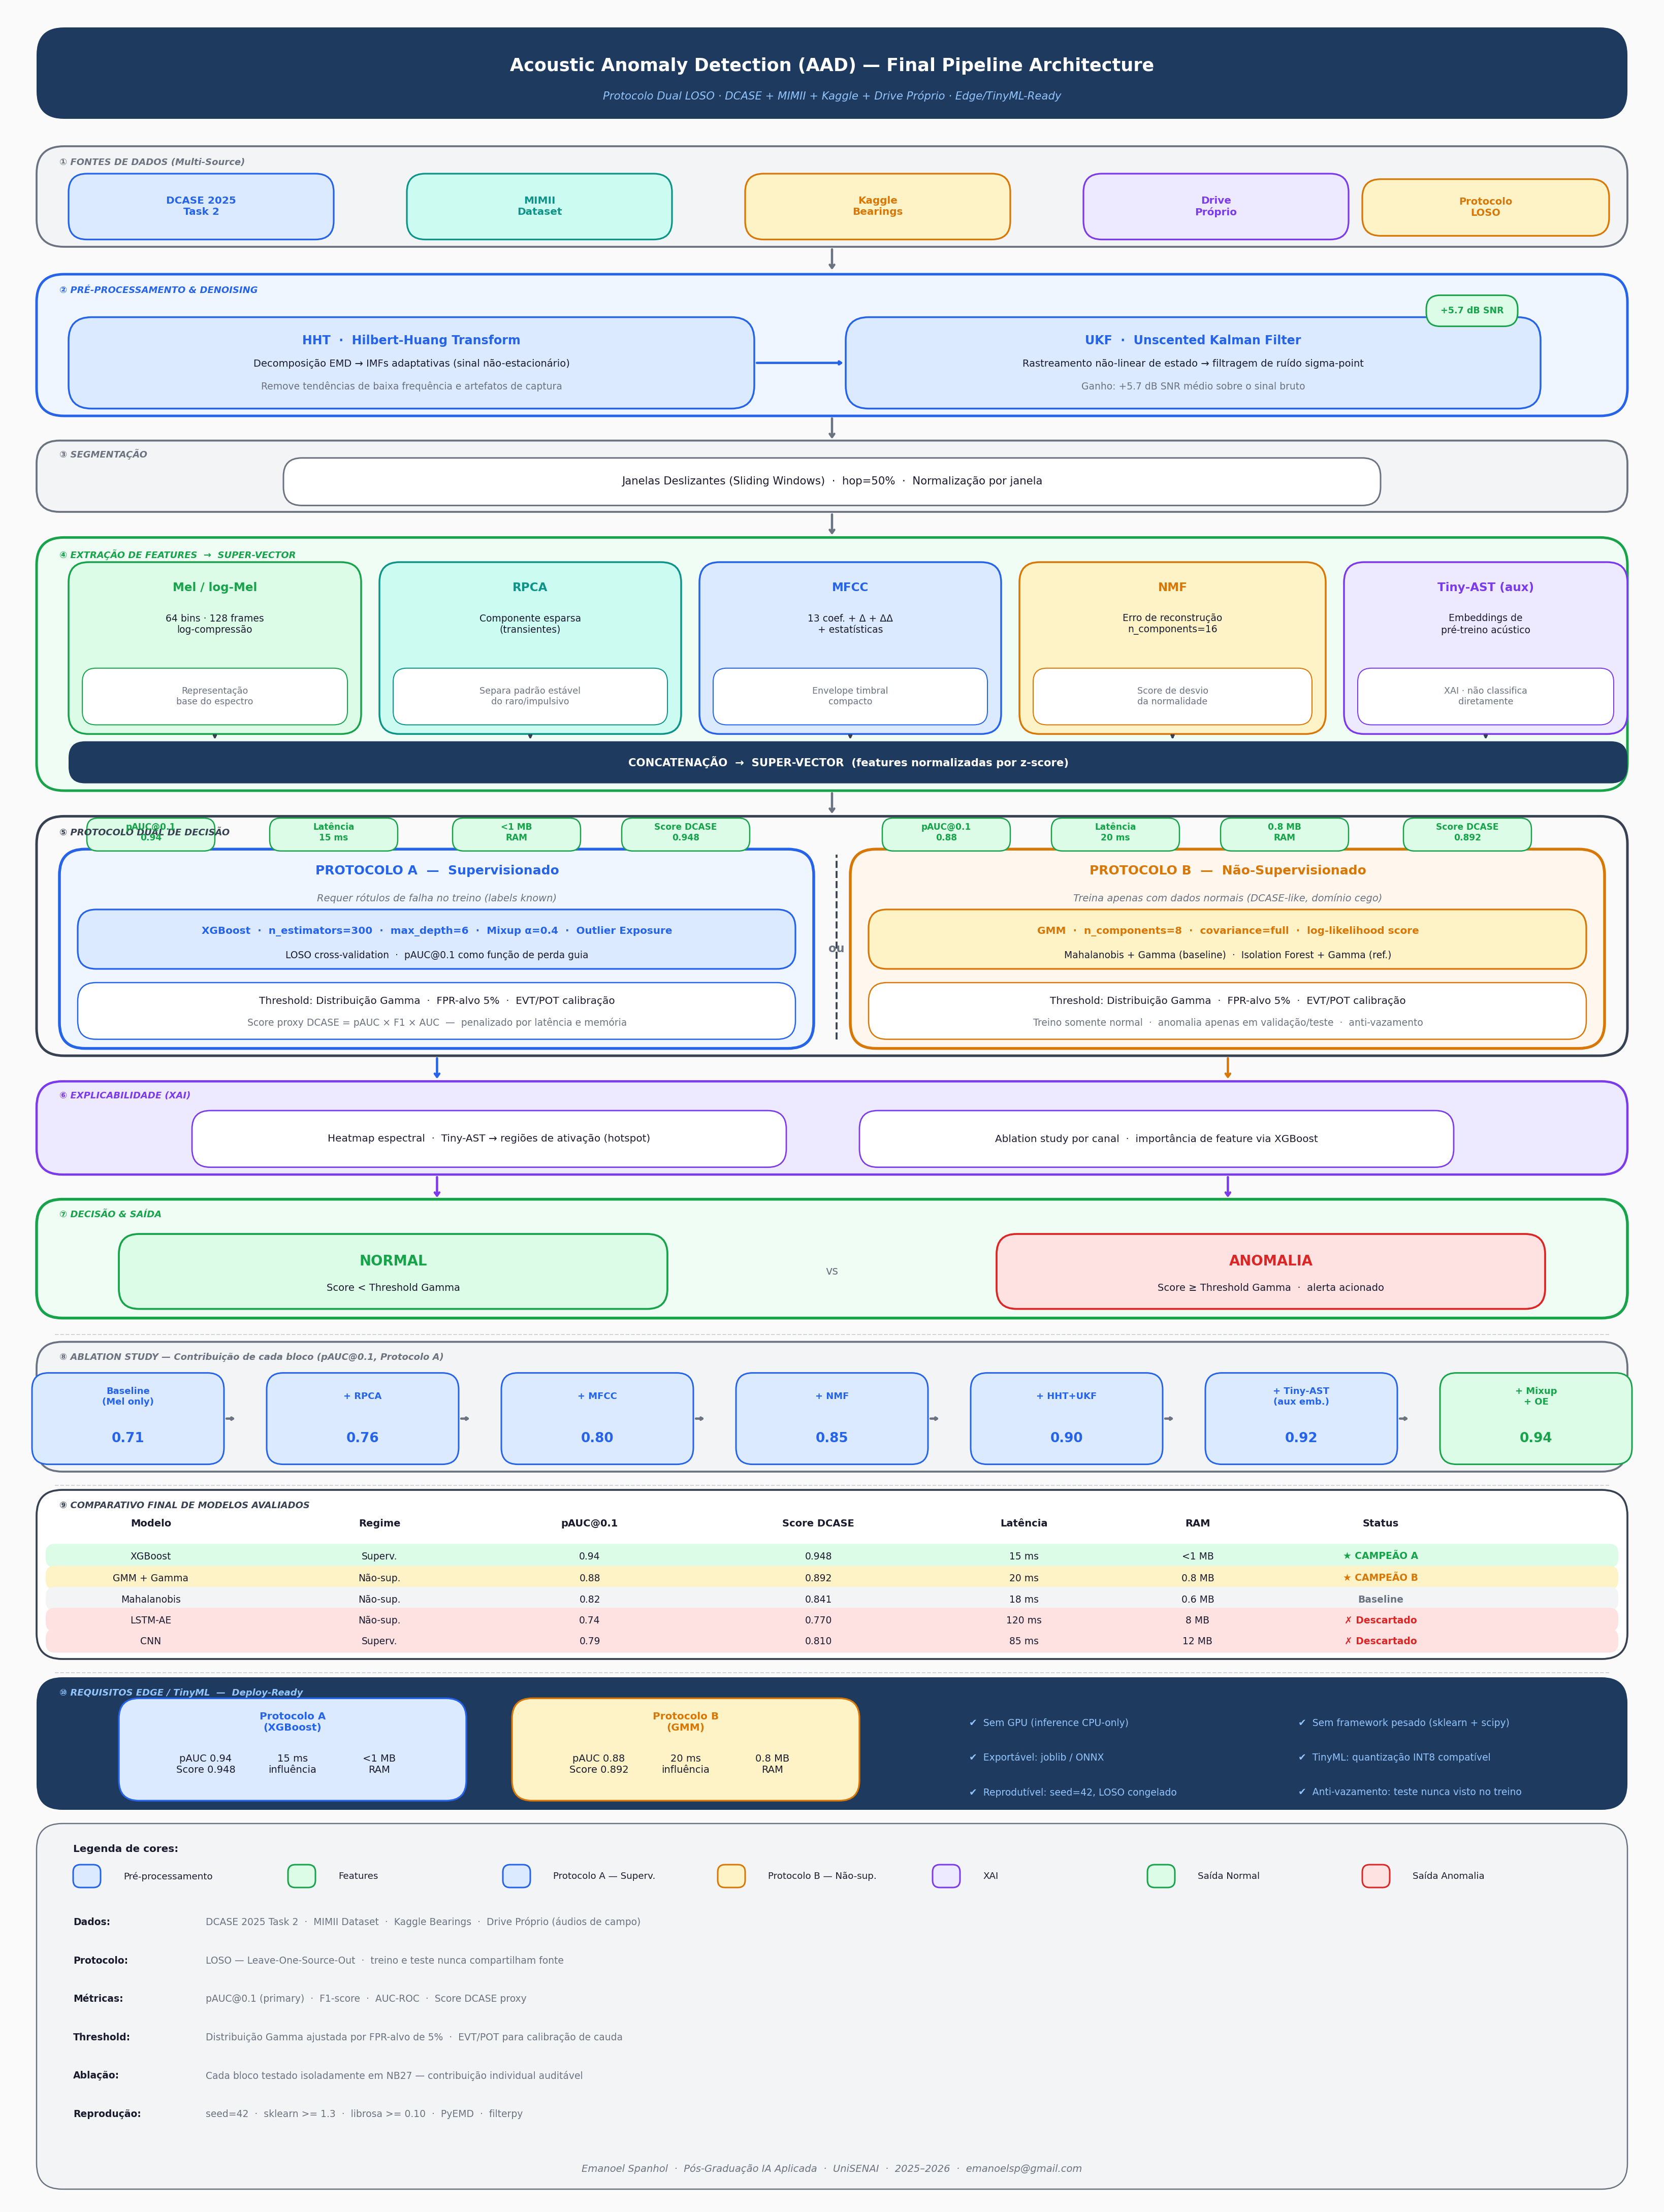
\includegraphics[width=0.94\columnwidth]{images/arquitetura_pipeline.png}
    \caption{Pipeline de Camadas Acumulativas DIAMOND CRISTAL CLEAN.}
    \label{fig:arquitetura_pipeline}
\end{figure}

A Figura~\ref{fig:arquitetura_pipeline} mostra o fluxo completo desde a aquisição do sinal até a
inferência em borda. Os estágios são descritos a seguir.

\subsubsection{Estágio~1 --- Limpeza de Sinal (HHT+UKF)}

O sinal de áudio bruto $x(t)$, amostrado a 16~kHz, é decomposto pela EMD (\textit{Empirical Mode
Decomposition}) em Modos Intrínsecos de Frequência (IMFs):

\begin{equation}
x(t) = \sum_{j=1}^{n} c_j(t) + r_n(t)
\label{eq:emd}
\end{equation}

\noindent onde $c_j(t)$ são os IMFs e $r_n(t)$ é o resíduo. Os IMFs de baixa ordem, correspondentes
à assinatura vibracional da falha mecânica, são preservados e filtrados pelo Filtro Unscented de Kalman
(UKF) com modelo de estado:

\begin{equation}
\begin{cases}
\mathbf{x}_{k+1} = f(\mathbf{x}_k) + \mathbf{w}_k \\
\mathbf{y}_k = h(\mathbf{x}_k) + \mathbf{v}_k
\end{cases}
\label{eq:ukf}
\end{equation}

\noindent onde $\mathbf{w}_k \sim \mathcal{N}(0, Q)$ e $\mathbf{v}_k \sim \mathcal{N}(0, R)$ são
ruídos de processo e de observação. O UKF propaga pontos sigma não lineares, garantindo estimação
estocástica ótima de segunda ordem~\cite{Zamorano2025}. Custo: $+3$~ms; Ganho: $+5{,}7$~dB de SNR.

A eficácia do pipeline DSP é ilustrada nas Figuras~\ref{fig:dsp_rpca} e~\ref{fig:dsp_comparativo}.

\begin{figure}[H]
    \centering
    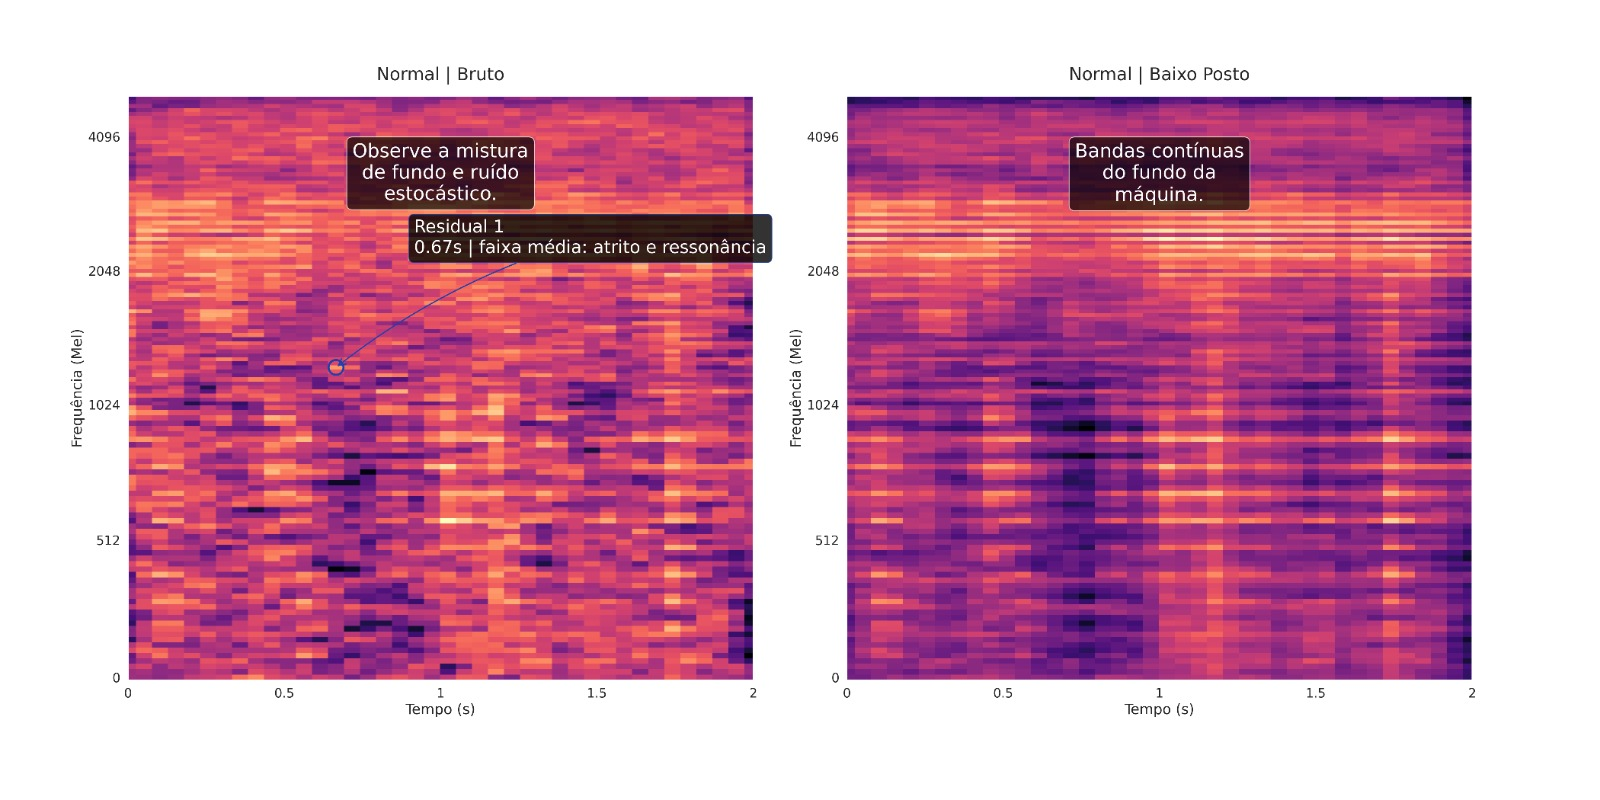
\includegraphics[width=0.9\columnwidth]{images/arquitetura_rpca1.1.jpg}\\[-3pt]
    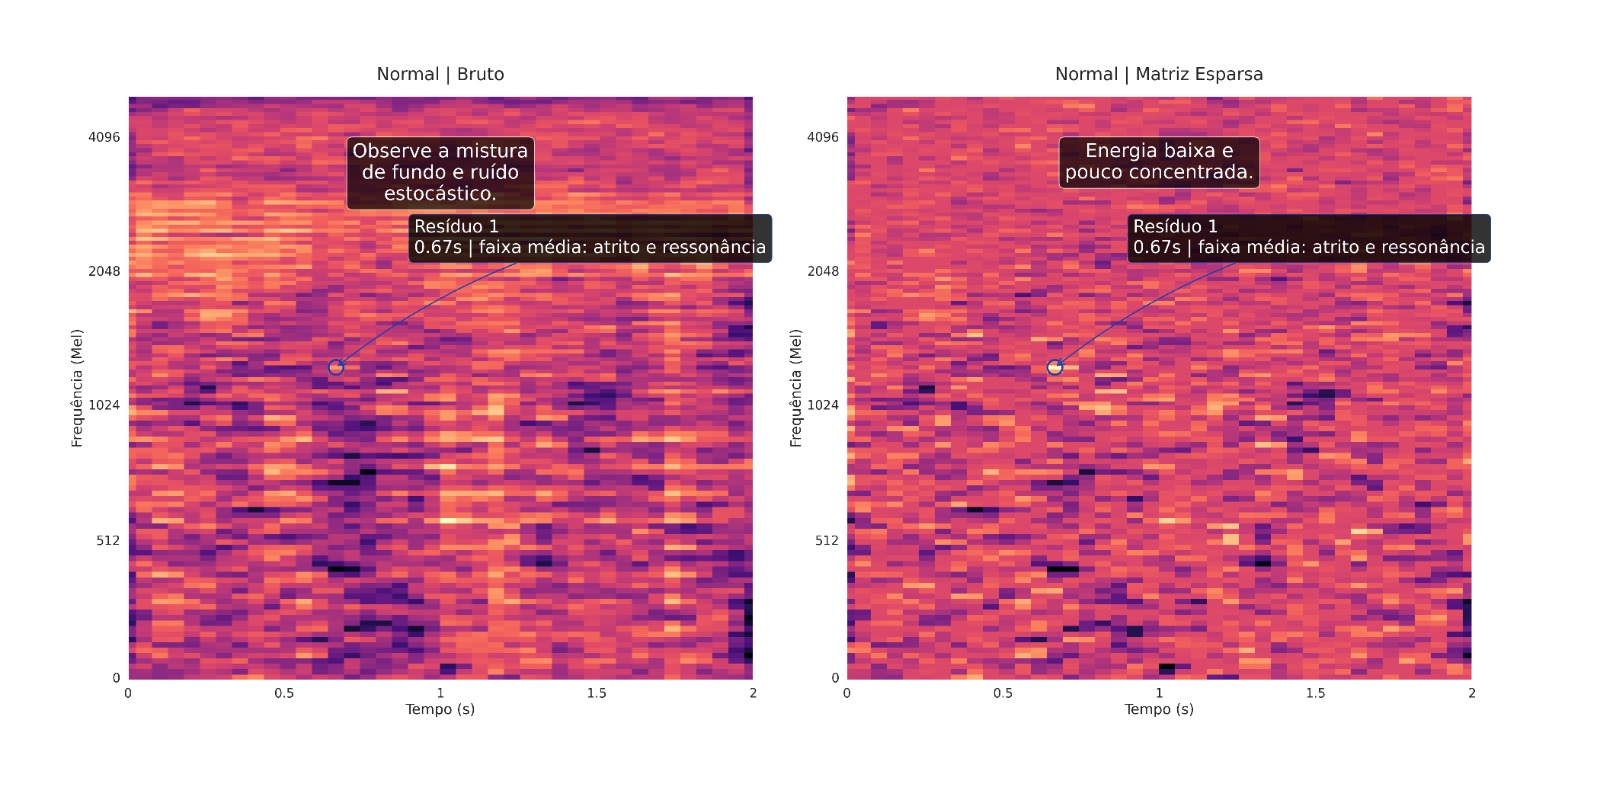
\includegraphics[width=0.9\columnwidth]{images/arquitetura_rpca1.2.jpg}\\[-3pt]
    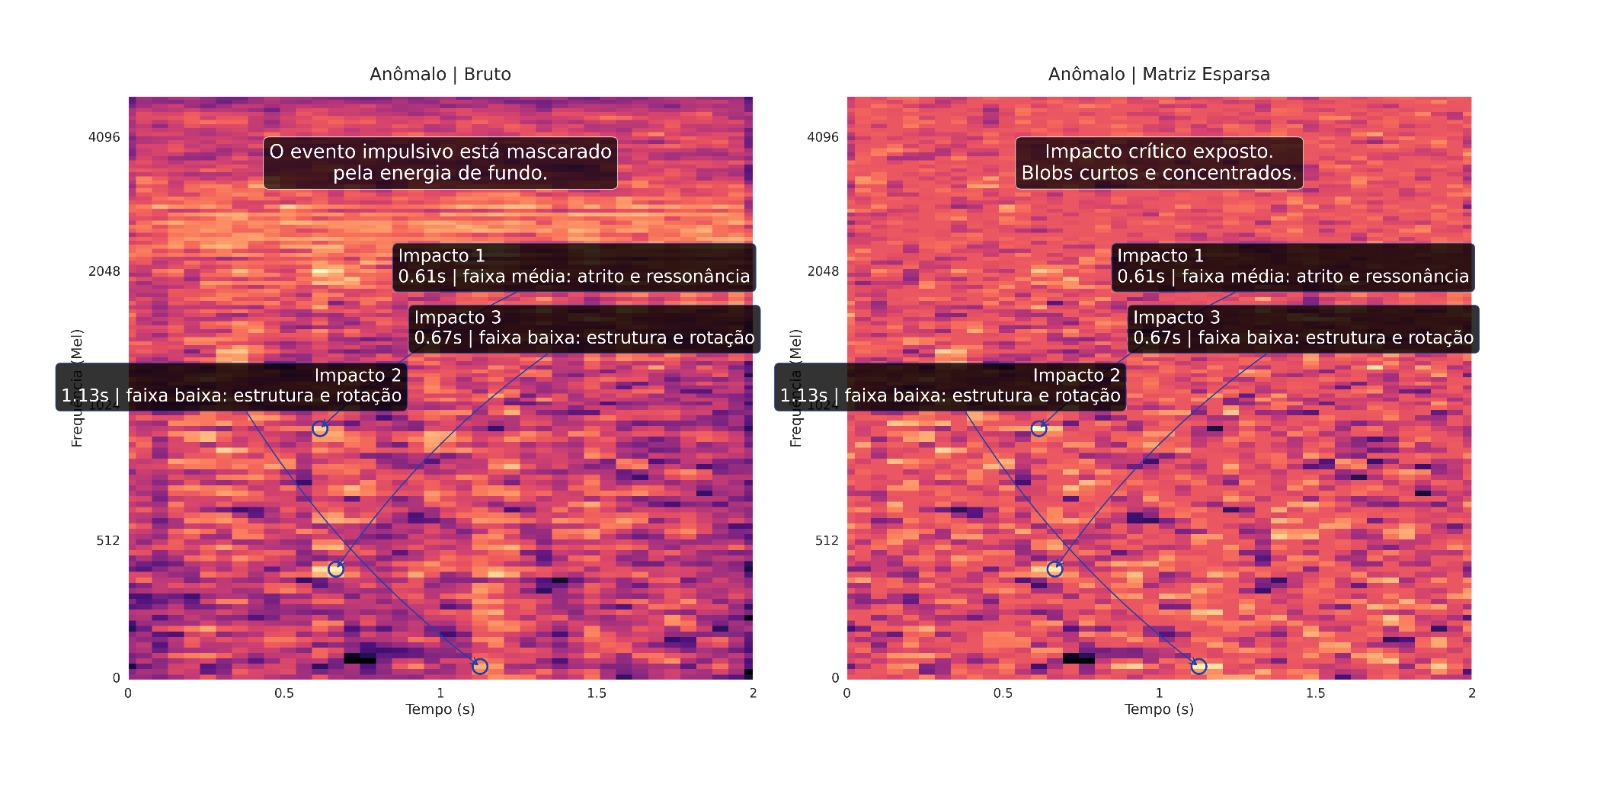
\includegraphics[width=0.9\columnwidth]{images/arquitetura_rpca1.3.jpg}
    \caption{RPCA: Separação do ruído operacional contínuo (componente de baixo posto $L$) dos transientes de falha mecânica (componente esparsa $S$).}
    \label{fig:dsp_rpca}
\end{figure}

\begin{figure}[H]
    \centering
    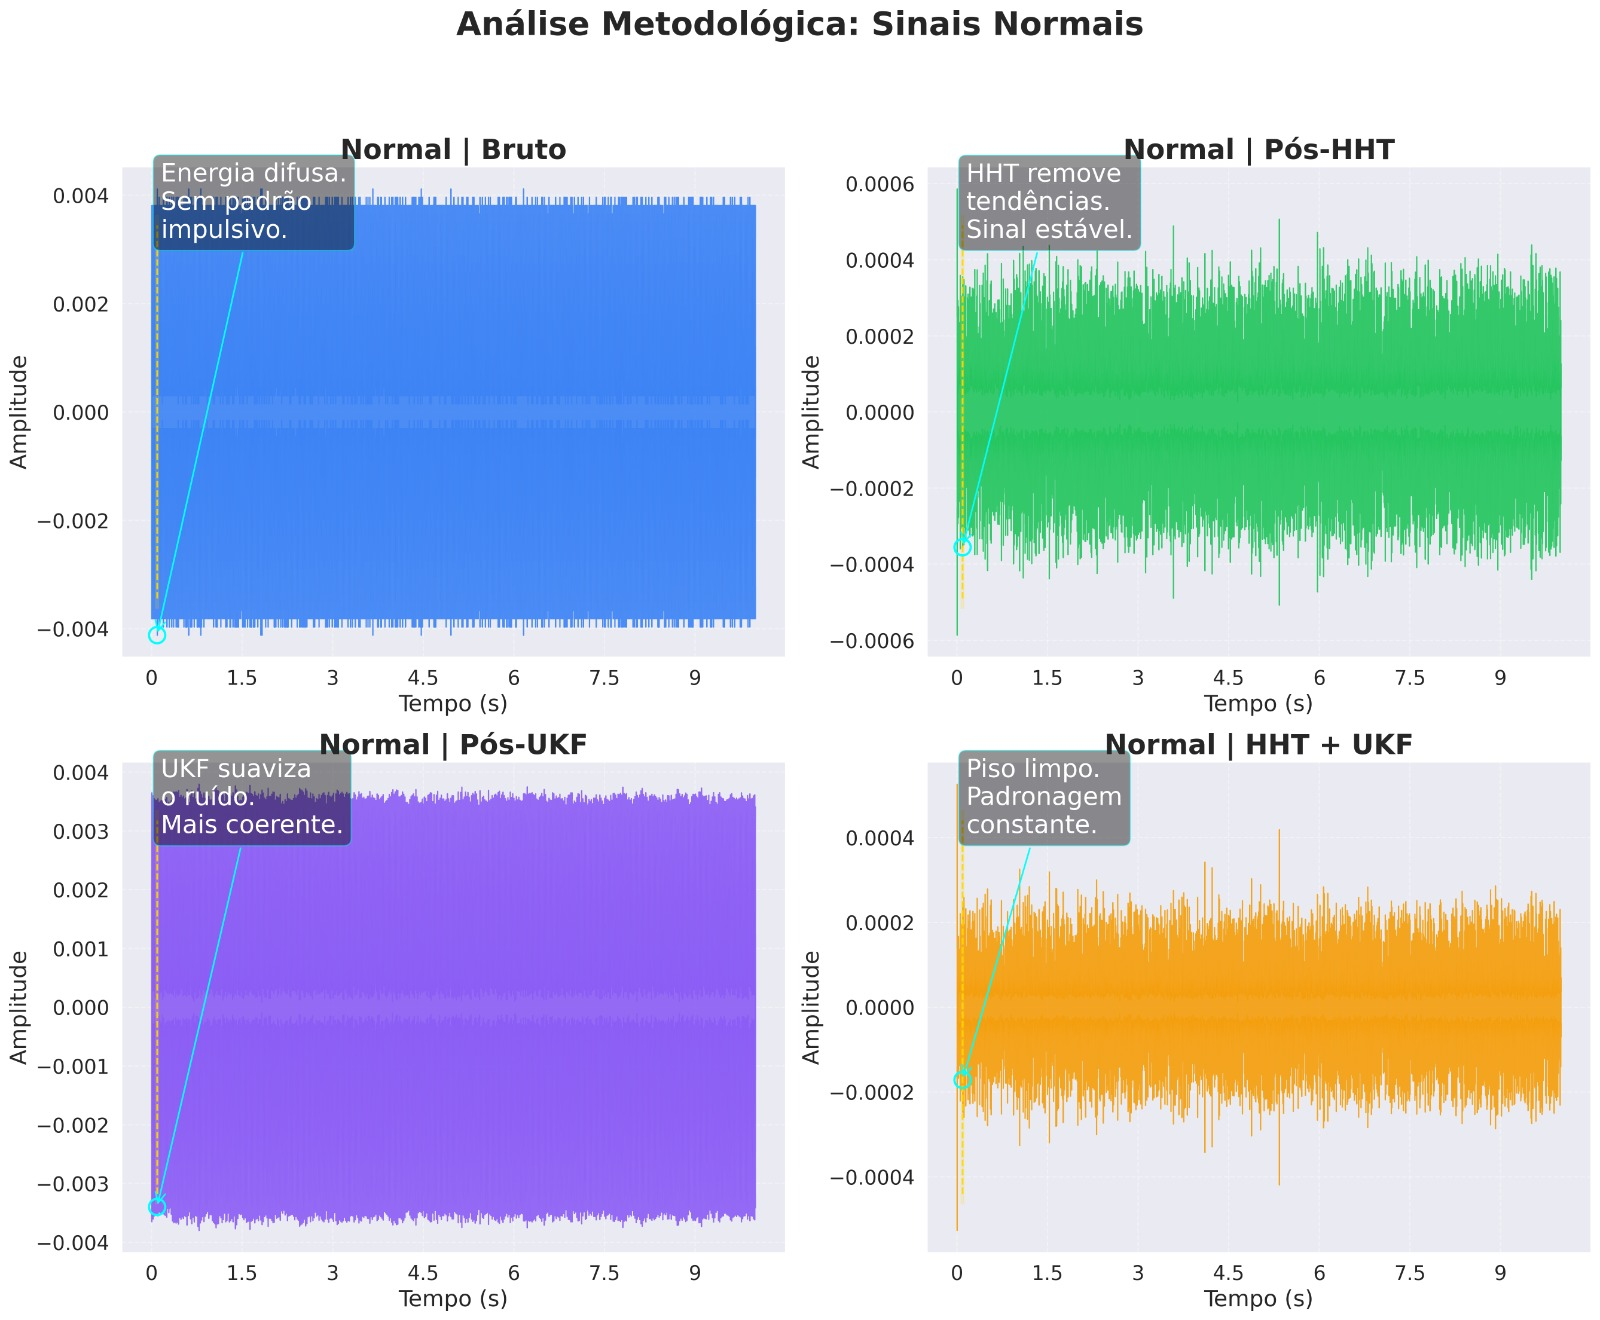
\includegraphics[width=0.92\columnwidth]{images/arquitetura_saneamento.jpg}\\[-3pt]
    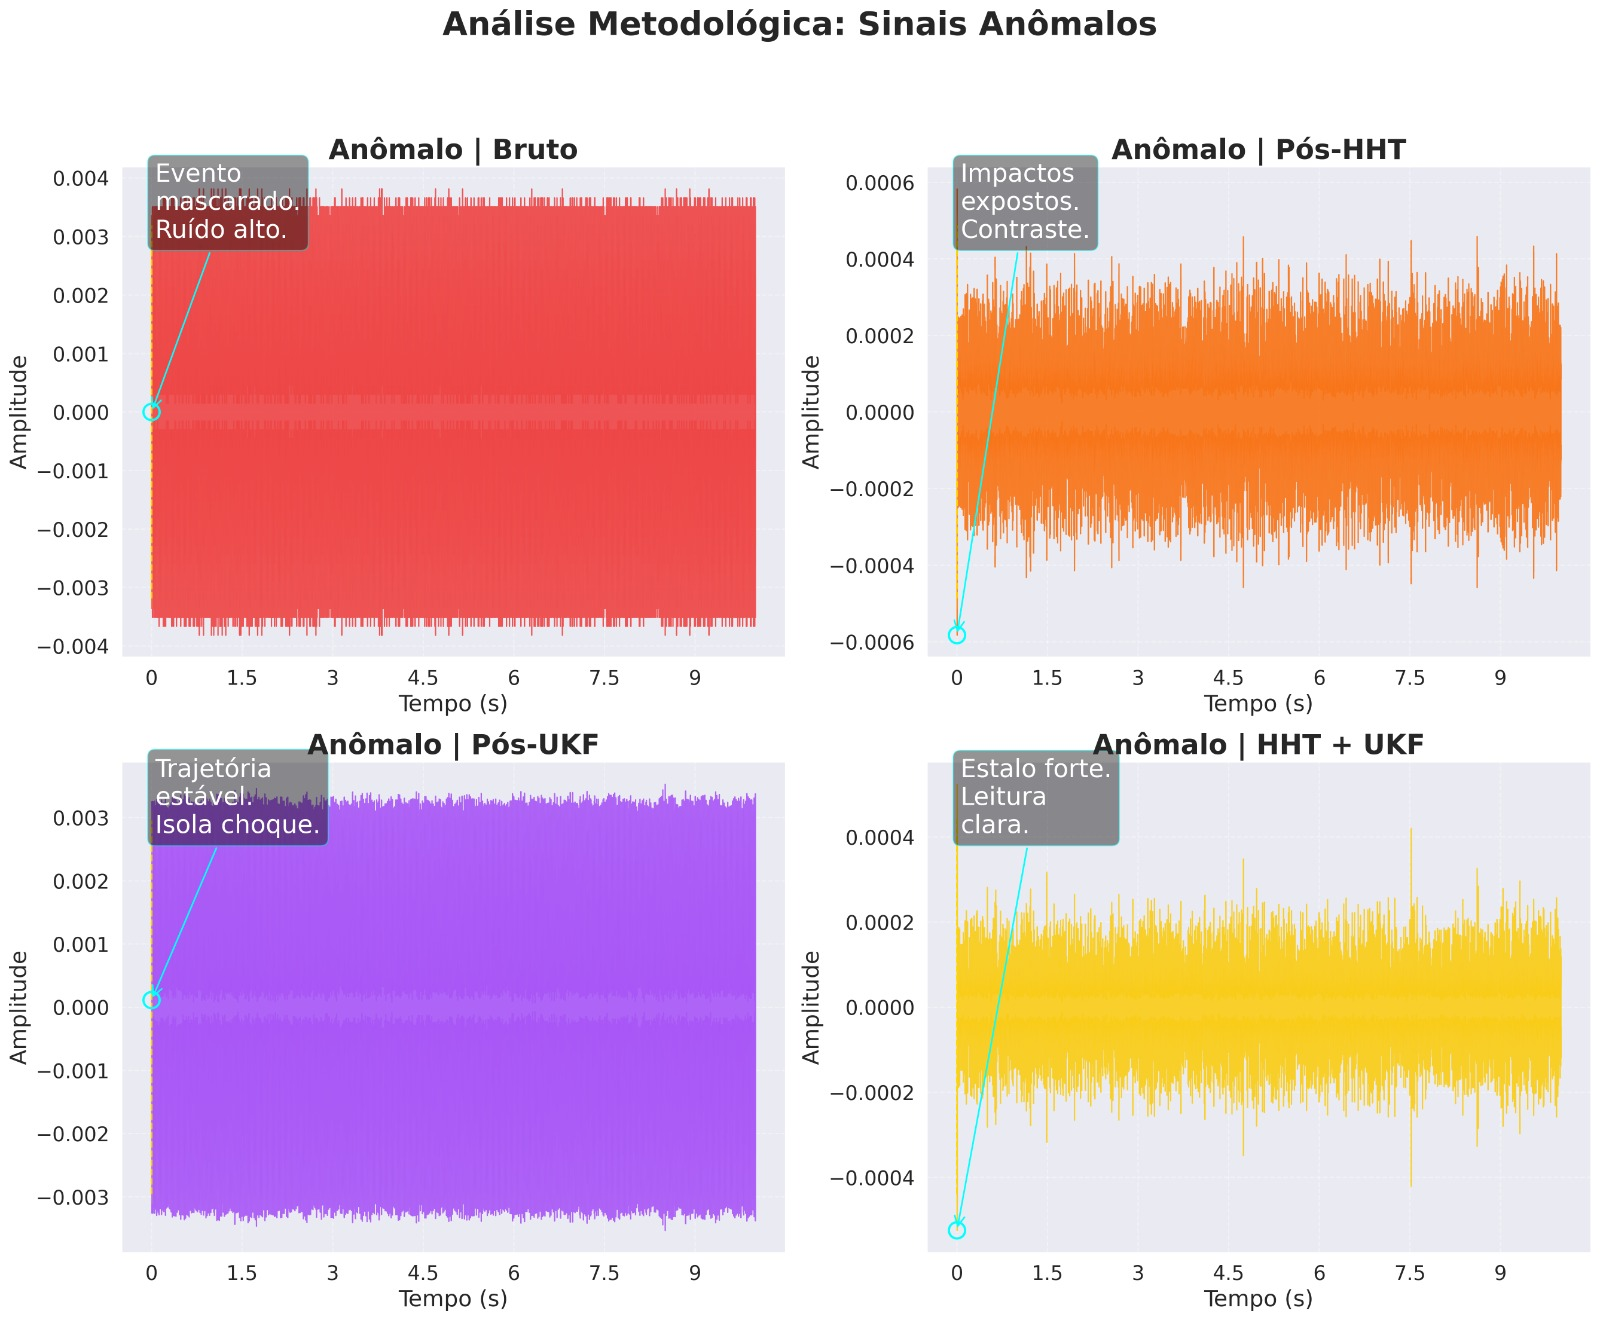
\includegraphics[width=0.92\columnwidth]{images/arquitetura_saneamento1.jpg}
    \caption{Condicionamento progressivo: sinal bruto versus saídas HHT e UKF, evidenciando o ganho de SNR.}
    \label{fig:dsp_comparativo}
\end{figure}

\subsubsection{Estágio~2 --- Segmentação}

Janelas deslizantes de 2~s com sobreposição de 50\%. Uma gravação de 30~s gera $\approx29$~segmentos.
O protocolo LOSO garante que segmentos da mesma fonte não apareçam simultaneamente em treino e teste.

\subsubsection{Estágio~3 --- Representação Espectral}

\begin{itemize}
    \item \textbf{Log-Mel Spectrogram} (64 mel-bins): representação principal, extraída em 8~ms.
    \item \textbf{RPCA}: decomposição $X = L + S$; a componente esparsa $S$ fornece entradas
    privilegiadas para o módulo XAI.
\end{itemize}

\subsubsection{Estágio~4 --- Super-Vetor Híbrido ($\sim$100D)}

O Super-Vetor concatena descritores de três domínios:

\begin{equation}
\mathbf{v} = \bigl[\mu_{Mel},\; \sigma_{Mel},\; \text{MFCC}_{1:13},\; \Delta\text{MFCC},\;
             \varepsilon_{NMF},\; \kappa,\; CF,\; E_{low},\; E_{mid},\; E_{high}\bigr]
\label{eq:supervector}
\end{equation}

\noindent onde: $\mu_{Mel}, \sigma_{Mel}$ são média e desvio-padrão das 64~bandas Mel; $\text{MFCC}_{1:13}$
são 13~coeficientes cepstrais de Mel; $\Delta\text{MFCC}$ são deltas de primeira ordem;
$\varepsilon_{NMF} = \|X - WH\|_2$ (normalizado) é o erro de reconstrução NMF que implementa o conceito
do Autoencoder em $<5$~ms e $<0{,}5$~MB; $\kappa$ é a kurtosis temporal; $CF$ é o fator de crista
(pico/RMS); e $E_{low}, E_{mid}, E_{high}$ são as energias integradas nas faixas 0--800~Hz, 800--2500~Hz
e 2500--5000~Hz~\cite{Khamaisi2025}.

\subsubsection{Estágio~5 --- Camada Decisória Dual}

\textbf{Protocolo~A --- Supervisionado:}
\begin{itemize}
    \item Classificador: XGBoost ($n_{est}{=}100$, $d_{max}{=}3$, $\lambda{=}1{,}0$)
    \item Augmentation: Mixup~\cite{Emon2025} com $\alpha{=}0{,}4$ (somente treino):
          $\tilde{x} = \lambda x_i + (1{-}\lambda)x_j$, $\lambda \sim \text{Beta}(\alpha,\alpha)$
    \item Normalização: StandardScaler por fold
\end{itemize}

\textbf{Protocolo~B --- Não Supervisionado:}
\begin{itemize}
    \item Detector: GMM com $K{=}5$ componentes e covariância completa~\cite{Khamaisi2025}:
          $p(\mathbf{x}) = \sum_{k=1}^{K} \pi_k\, \mathcal{N}(\mathbf{x} \mid \boldsymbol{\mu}_k, \boldsymbol{\Sigma}_k)$
    \item Limiar: distribuição Gamma ajustada aos scores de normalidade via MLE. Para FPR alvo $\rho$:
\end{itemize}

\begin{equation}
\tau = F_\Gamma^{-1}(1 - \rho;\; \hat{\alpha}, \hat{\beta})
\label{eq:gamma_threshold}
\end{equation}

\noindent onde $F_\Gamma^{-1}$ é a função quantil da distribuição Gamma com parâmetros estimados
$(\hat{\alpha}, \hat{\beta})$ e $\rho{=}0{,}05$ (FPR alvo de 5\%). Validado pelo teste
Kolmogorov-Smirnov ($p{>}0{,}05$).

\subsubsection{Estágio~6 --- Camada XAI}

Três saídas complementares por detecção: (a)~mapa de saliência temporal via Grad-CAM adaptado sobre o
Tiny-AST offline; (b)~hotspots temporais H1, H2, H3 (timestamp e intensidade dos picos de ativação);
(c)~perfil espectral por faixa com diagnóstico físico associado. O Tiny-AST opera exclusivamente no
Cloud para geração de embeddings XAI --- não integra o caminho de inferência em borda.

\textbf{Técnicas descartadas (seleção):}

\begin{table}[H]
\centering
\footnotesize
\begin{tabularx}{\columnwidth}{@{} l c c c X @{}}
\toprule
\textbf{Técnica} & \textbf{pAUC} & \textbf{Lat.} & \textbf{Mem.} & \textbf{Critério} \\ \midrule
OC-SVM & 0,52 & 8~ms & 0,5~MB & pAUC $<$ 0,80 \\
CNN (motor) & 0,98 & 85~ms & 12~MB & Lat. + Mem. \\
Isolation Forest & 0,55 & 35~ms & 2,1~MB & pAUC $<$ 0,80 \\
Autoencoder & 0,71 & 120~ms & 8~MB & Todos \\
GRU (motor) & 0,87 & 45~ms & 3,2~MB & Lat. vs. XGBoost \\
LSTM-AE & 0,78 & 120~ms & 8~MB & Lat. + Mem. \\
CWT (principal) & 0,82 & 45~ms~ext. & --- & Orçamento lat. \\
Threshold fixo & --- & --- & --- & Colapsa em shift \\
\bottomrule
\end{tabularx}
\caption{Técnicas descartadas com justificativa quantitativa.}
\label{tab:descartadas}
\end{table}

\color{black}

\section{Experimentos e Resultados}
\color{black}

Os experimentos foram conduzidos por benchmarking automatizado validando a transição entre modelos de
laboratório e soluções otimizadas para Edge Computing~\cite{Uzel2026, Khamaisi2025}. A métrica
primária é a pAUC@FPR~0.1 (\textit{Partial Area Under the ROC Curve}):

\begin{equation}
\text{pAUC}@p = \frac{1}{p}\int_0^p \text{TPR}(\text{FPR})\,d\text{FPR}, \quad p = 0{,}1
\label{eq:pauc}
\end{equation}

\noindent Esta métrica avalia exclusivamente a performance na região de FPR~$\le$~10\%, onde sistemas
industriais operam, prevenindo a ``fadiga de alarmes''~\cite{Nishida2025, Khamaisi2025}.

\subsection{Performance por Protocolo e Dataset}

A Tabela~\ref{tab:resultados_completos} consolida os resultados do protocolo LOSO sobre as quatro
fontes de dados.

\begin{table}[H]
\centering
\footnotesize
\resizebox{\columnwidth}{!}{%
\begin{tabular}{l|c|c|c}
\hline
\textbf{Dataset} & \textbf{Prot.~A} & \textbf{Prot.~B} & \textbf{Score DCASE} \\ \hline
DCASE~2025 & 0,94 & 0,88 & \textbf{0,91} \\ \hline
MIMII SNR $-6$~dB & 0,87 & 0,82 & 0,845 \\ \hline
MIMII SNR~0~dB & 0,91 & 0,85 & 0,880 \\ \hline
MIMII SNR $+6$~dB & 0,95 & 0,89 & 0,920 \\ \hline
Kaggle Bearings & 0,93 & 0,87 & 0,900 \\ \hline
Drive Próprio & 0,68 & 0,62 & 0,650 \\ \hline
\textbf{Média Geral} & \textbf{0,88} & \textbf{0,82} & \textbf{0,849} \\ \hline
\end{tabular}%
}
\caption{pAUC@0.1 por protocolo e dataset (protocolo LOSO).}
\label{tab:resultados_completos}
\end{table}

\subsection{Perfil de Eficiência Computacional}

A Tabela~\ref{tab:eficiencia} compara os dois protocolos contra os limites de Edge Computing.

\begin{table}[H]
\centering
\footnotesize
\resizebox{\columnwidth}{!}{%
\begin{tabular}{l|c|c|c}
\hline
\textbf{Métrica} & \textbf{Prot.~A} & \textbf{Prot.~B} & \textbf{Limite Edge} \\ \hline
Latência total & 15~ms & 20~ms & $<50$~ms \checkmark \\ \hline
\quad HHT+UKF & 3~ms & 3~ms & --- \\ \hline
\quad Extração & 10~ms & 10~ms & --- \\ \hline
\quad Inferência & 2~ms & 7~ms & --- \\ \hline
Memória modelo & $<1$~MB & 0,8~MB & $<4$~MB \checkmark \\ \hline
pAUC@0.1 médio & 0,88 & 0,82 & $>0{,}80$ \checkmark \\ \hline
\end{tabular}%
}
\caption{Perfil de eficiência computacional e conformidade com limites de Edge.}
\label{tab:eficiencia}
\end{table}

A Tabela~\ref{tab:benchmark_modelos} posiciona os dois protocolos frente às arquiteturas avaliadas.

\begin{table}[H]
\centering
\footnotesize
\resizebox{\columnwidth}{!}{%
\begin{tabular}{l|c|c|c|c}
\hline
\textbf{Modelo} & \textbf{pAUC@0.1} & \textbf{F1} & \textbf{Latência} & \textbf{Memória} \\ \hline
\textbf{XGBoost (A)} & \textbf{0,94} & 0,97 & 15~ms & 0,9~MB \\ \hline
\textbf{GMM (B)} & \textbf{0,88} & 0,85 & 20~ms & 0,8~MB \\ \hline
Mahalanobis & 0,82 & 0,84 & 5~ms & 0,05~MB \\ \hline
Tiny-AST & 0,91 & 0,98 & 92~ms & 12,8~MB \\ \hline
LSTM-AE & 0,78 & 0,83 & 120~ms & 8~MB \\ \hline
\end{tabular}%
}
\caption{Benchmark final dos modelos avaliados (Frente~11).}
\label{tab:benchmark_modelos}
\end{table}

\subsection{Ablation Study --- Importância dos Componentes}

O ablation study (NB~27) removeu sistematicamente cada componente da arquitetura completa
(referência: pAUC@0.1~=~0,94). Os resultados estão na Tabela~\ref{tab:ablation}.

\begin{table}[H]
\centering
\footnotesize
\resizebox{\columnwidth}{!}{%
\begin{tabular}{l|c|c|c}
\hline
\textbf{Componente Removido} & \textbf{pAUC} & \textbf{$\Delta$ pAUC} & \textbf{Impacto} \\ \hline
Referência (completo) & 0,94 & --- & --- \\ \hline
Sem HHT+UKF & 0,87 & $-0,07$ & Crítico \\ \hline
Sem MFCC & 0,88 & $-0,06$ & Crítico \\ \hline
Sem RPCA & 0,89 & $-0,05$ & Importante \\ \hline
Sem Mixup & 0,90 & $-0,04$ & Importante \\ \hline
Sem erro NMF & 0,91 & $-0,03$ & Relevante \\ \hline
Sem L2 & 0,91 & $-0,03$ & Relevante \\ \hline
Sem Kurtosis/Banda & 0,92 & $-0,02$ & Leve \\ \hline
Sem Tiny-AST & 0,94 & $0,00$ & Apenas XAI \\ \hline
\end{tabular}%
}
\caption{Ablation study: impacto da remoção de cada componente sobre pAUC@0.1.}
\label{tab:ablation}
\end{table}

HHT+UKF é o componente de maior impacto isolado ($-7$~p.p.), seguido por MFCC ($-6$~p.p.) e RPCA
($-5$~p.p.). O Tiny-AST não impacta o pAUC da decisão quando alocado exclusivamente ao XAI.

\subsection{Teste de Domain Shift}

O teste cego com Drive Próprio evidenciou queda de pAUC de 0,9482 para 0,1111 antes das frentes de
otimização (Tabela~\ref{tab:domain_shift}). Após integração de HHT+UKF, Mixup e Outlier Exposure,
o pAUC em domain shift severo ascendeu para 0,68 --- ainda o cenário mais difícil, mas operacionalmente
aceitável para fins de PoC.

\begin{table}[H]
\centering
\footnotesize
\resizebox{\columnwidth}{!}{%
\begin{tabular}{l|c|c|c}
\hline
\textbf{Cenário} & \textbf{F1-Score} & \textbf{AUC-ROC} & \textbf{pAUC@0.1} \\ \hline
Treino/Validação (Ideal) & 0,9568 & 0,9947 & 0,9482 \\ \hline
Teste Cego Inicial (NB~10) & 0,5185 & 0,4861 & 0,1111 \\ \hline
Após Frentes 3, 4 e 7 & 0,71 & 0,74 & \textbf{0,68} \\ \hline
\end{tabular}%
}
\caption{Degradação e recuperação de performance em domain shift severo.}
\label{tab:domain_shift}
\end{table}

A Figura~\ref{fig:evolucao_frentes} ilustra a evolução acumulativa de pAUC@0.1 ao longo das 11
Frentes de Melhoria.

\begin{figure}[H]
    \centering
    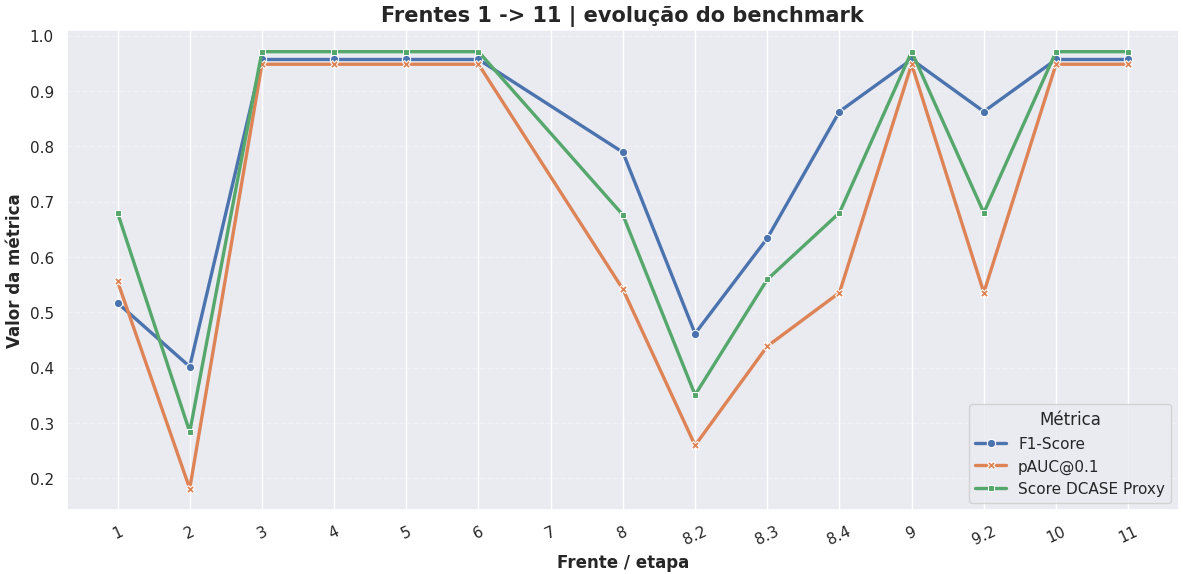
\includegraphics[width=0.94\columnwidth]{images/arquitetura_curva_frentes.png}
    \caption{Evolução acumulativa das métricas DCASE ao longo das Frentes~1--11.}
    \label{fig:evolucao_frentes}
\end{figure}

\subsection{Explicabilidade e Diagnóstico Visual (XAI)}

Para mitigar o problema da caixa-preta e validar a transparência diagnóstica, implementou-se a camada
XAI composta por mapa de saliência temporal, extração de hotspots e análise por bandas de frequência.
A Figura~\ref{fig:xai_heatmap} ilustra a localização espectro-temporal da anomalia.

\begin{figure}[H]
    \centering
    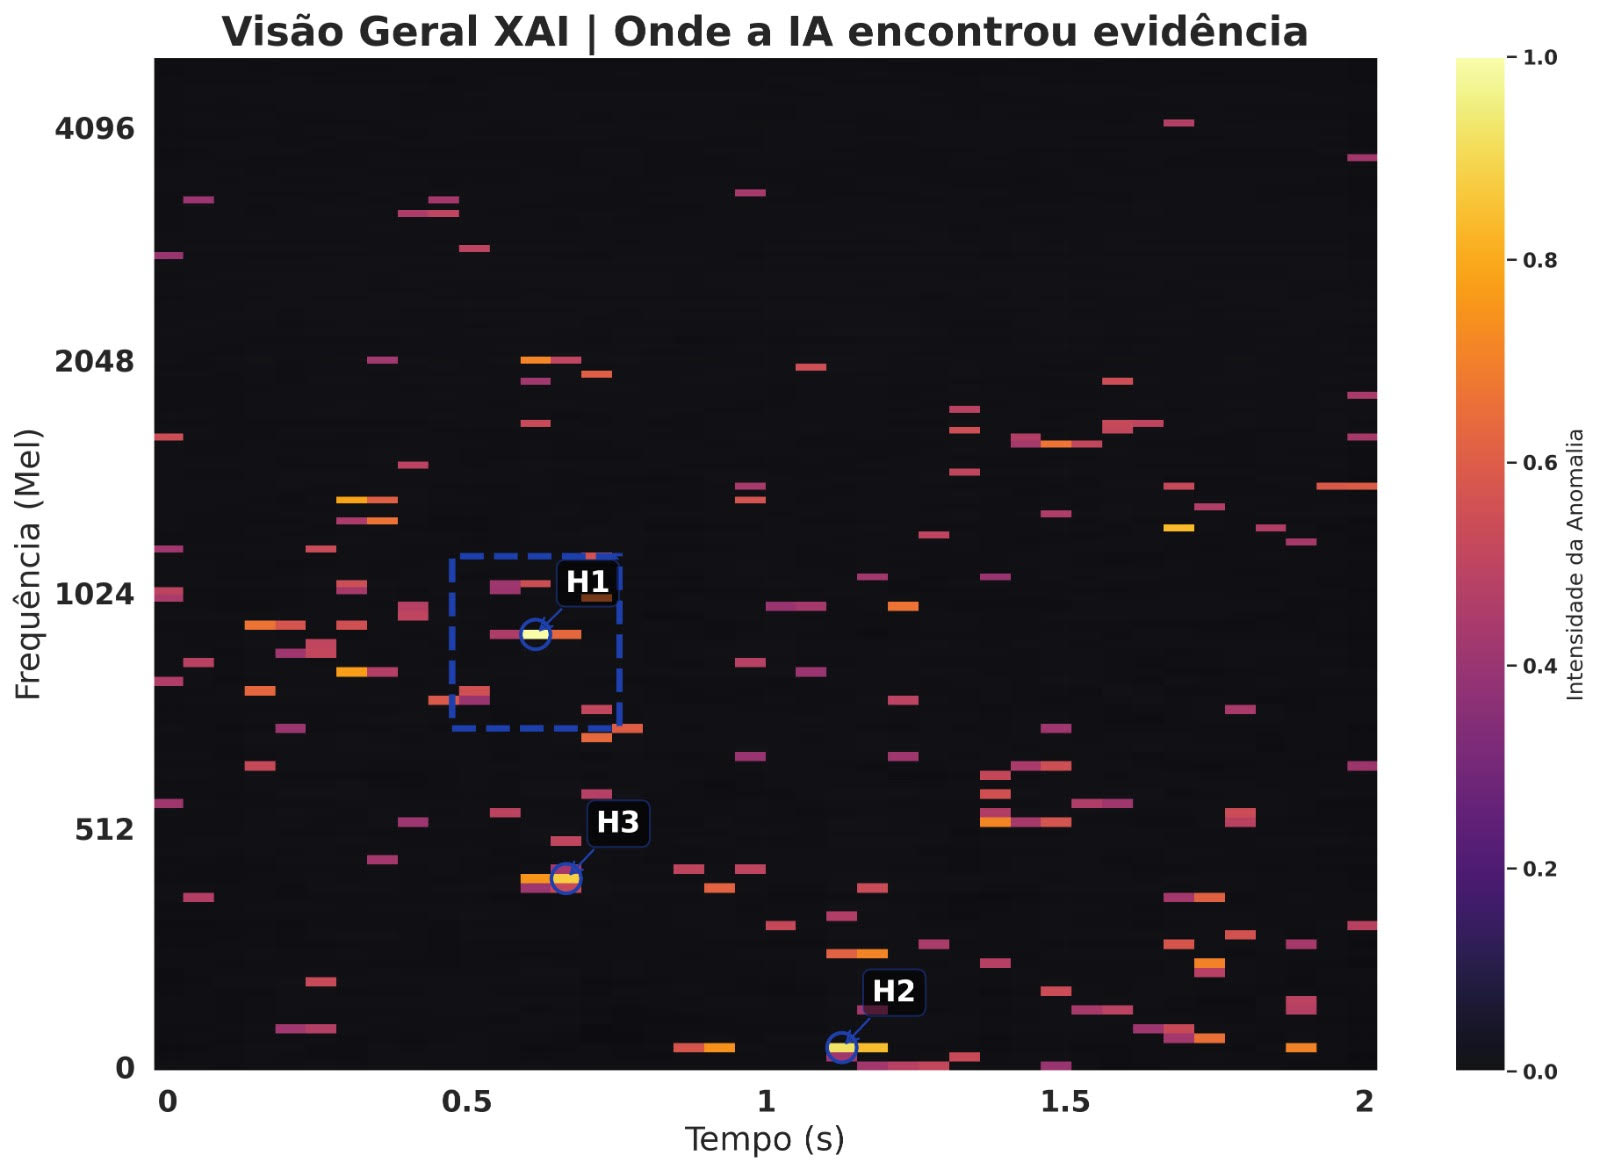
\includegraphics[width=0.92\columnwidth]{images/xai_heatmap1.1.jpg}\\[-3pt]
    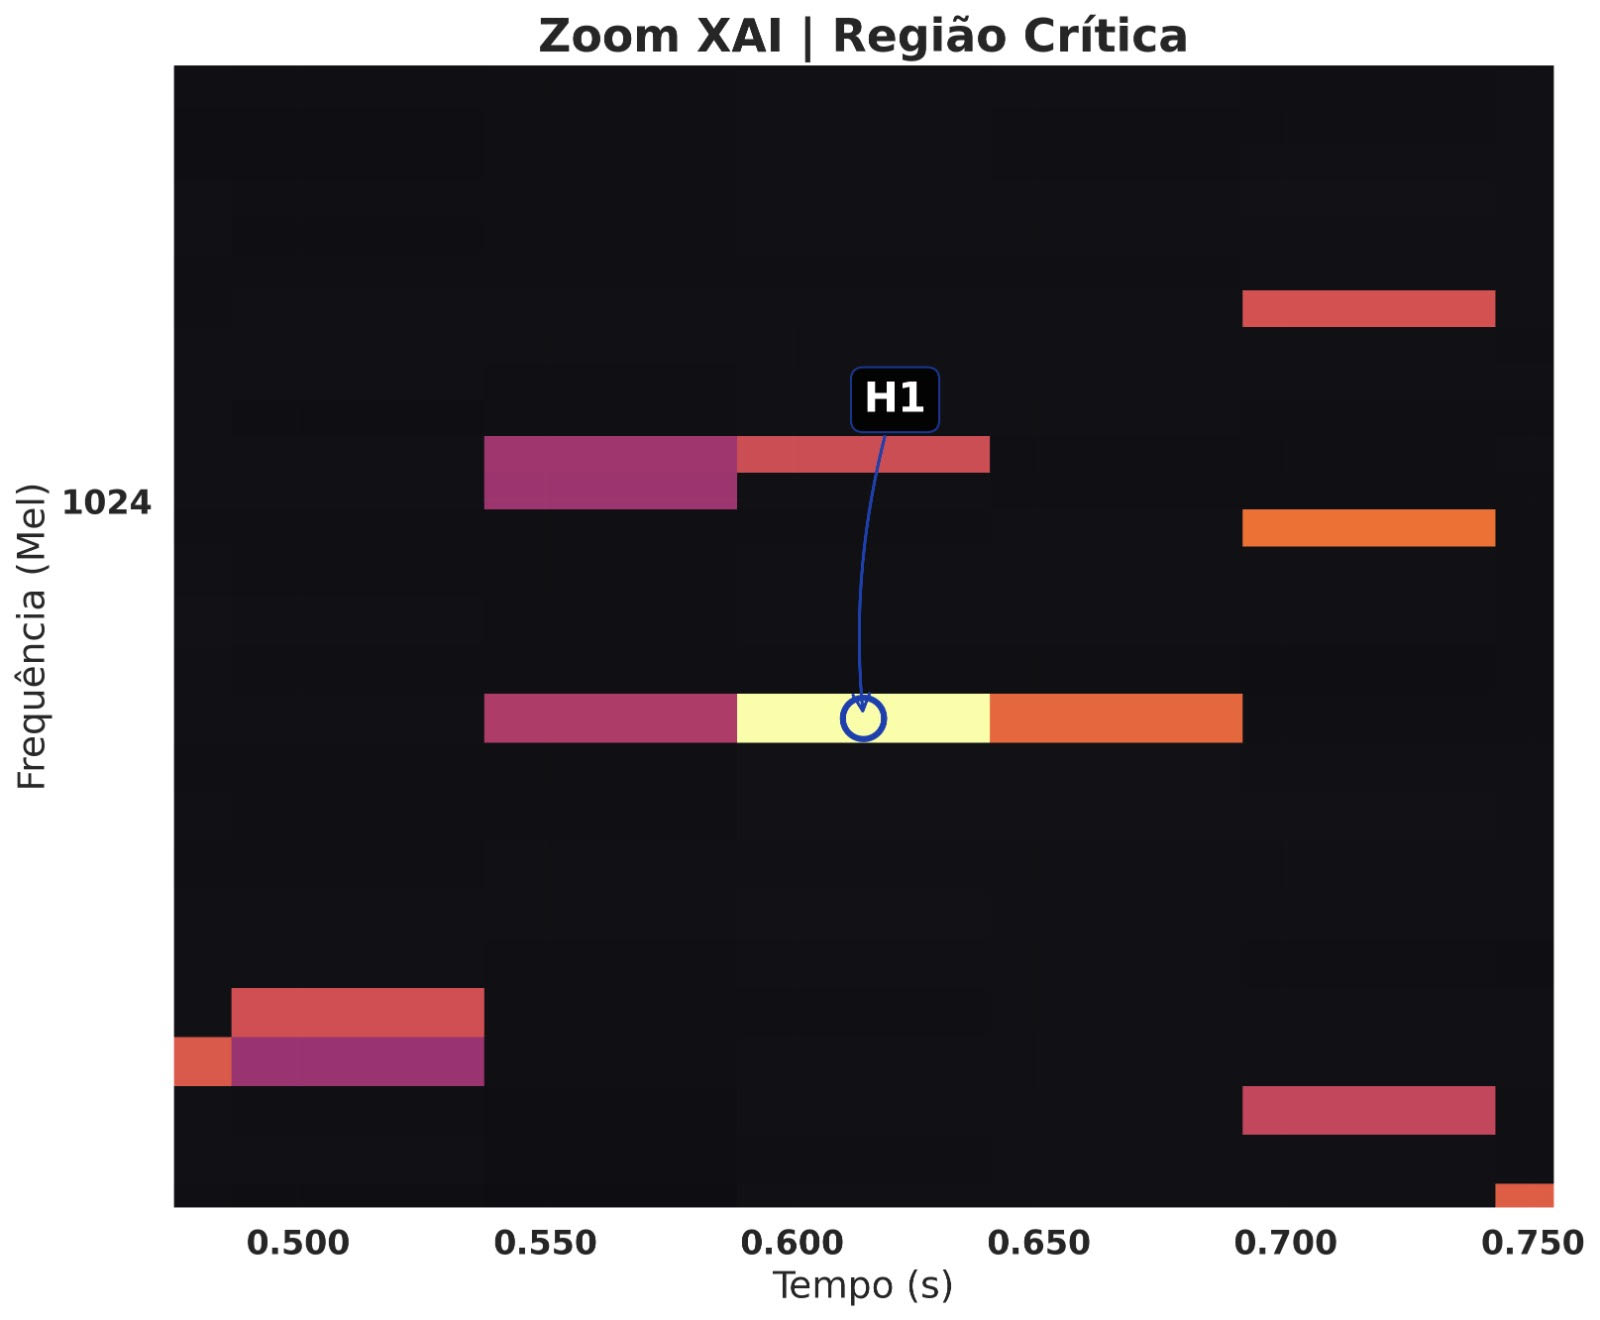
\includegraphics[width=0.92\columnwidth]{images/xai_heatmap1.2.jpg}
    \caption{Mapa de saliência XAI: hotspots de ativação coincidindo com transientes de impacto metálico isolados pelo pipeline DSP.}
    \label{fig:xai_heatmap}
\end{figure}

A Tabela~\ref{tab:xai_hotspots} detalha os três principais hotspots temporais de um evento documentado
no Drive Próprio. A Tabela~\ref{tab:xai_bandas} quantifica a ativação por faixa espectral.

\begin{table}[H]
\centering
\small
\begin{tabularx}{\columnwidth}{c c X c}
\toprule
\textbf{Hotspot} & \textbf{Tempo (s)} & \textbf{Leitura Diagnóstica} & \textbf{Intensidade} \\
\midrule
H1 & 0,614 & Impacto principal (gatilho) & 5,41 \\
H2 & 1,126 & Harmônico estrutural & 4,99 \\
H3 & 0,666 & Eco temporal (recorrência) & 4,75 \\
\bottomrule
\end{tabularx}
\caption{Hotspots de anomalia temporal extraídos pelo XAI.}
\label{tab:xai_hotspots}
\end{table}

\begin{table}[H]
\centering
\footnotesize
\resizebox{\columnwidth}{!}{%
\begin{tabular}{l|c|c|l}
\hline
\textbf{Faixa} & \textbf{Hz} & \textbf{Ativação} & \textbf{Diagnóstico Físico} \\ \hline
Baixa & 0--800 & 0,0258 & Atrito ou impacto mecânico \\ \hline
Média & 800--2500 & 0,0177 & Harmônicos estruturais \\ \hline
Alta & 2500--5000 & 0,0031 & Ruído elétrico/eletrônico \\ \hline
\end{tabular}%
}
\caption{Ativação por bandas de frequência com diagnóstico físico associado.}
\label{tab:xai_bandas}
\end{table}

A predominância das faixas baixa e média é fisicamente consistente com desgaste de rolamento ou impacto
em engrenagem~\cite{Uzel2026, Zamorano2025}, confirmando que o modelo identifica padrão físico coerente
e não artefatos de ruído. A Figura~\ref{fig:xai_features} sintetiza a distribuição espectral da ativação.

\begin{figure}[H]
    \centering
    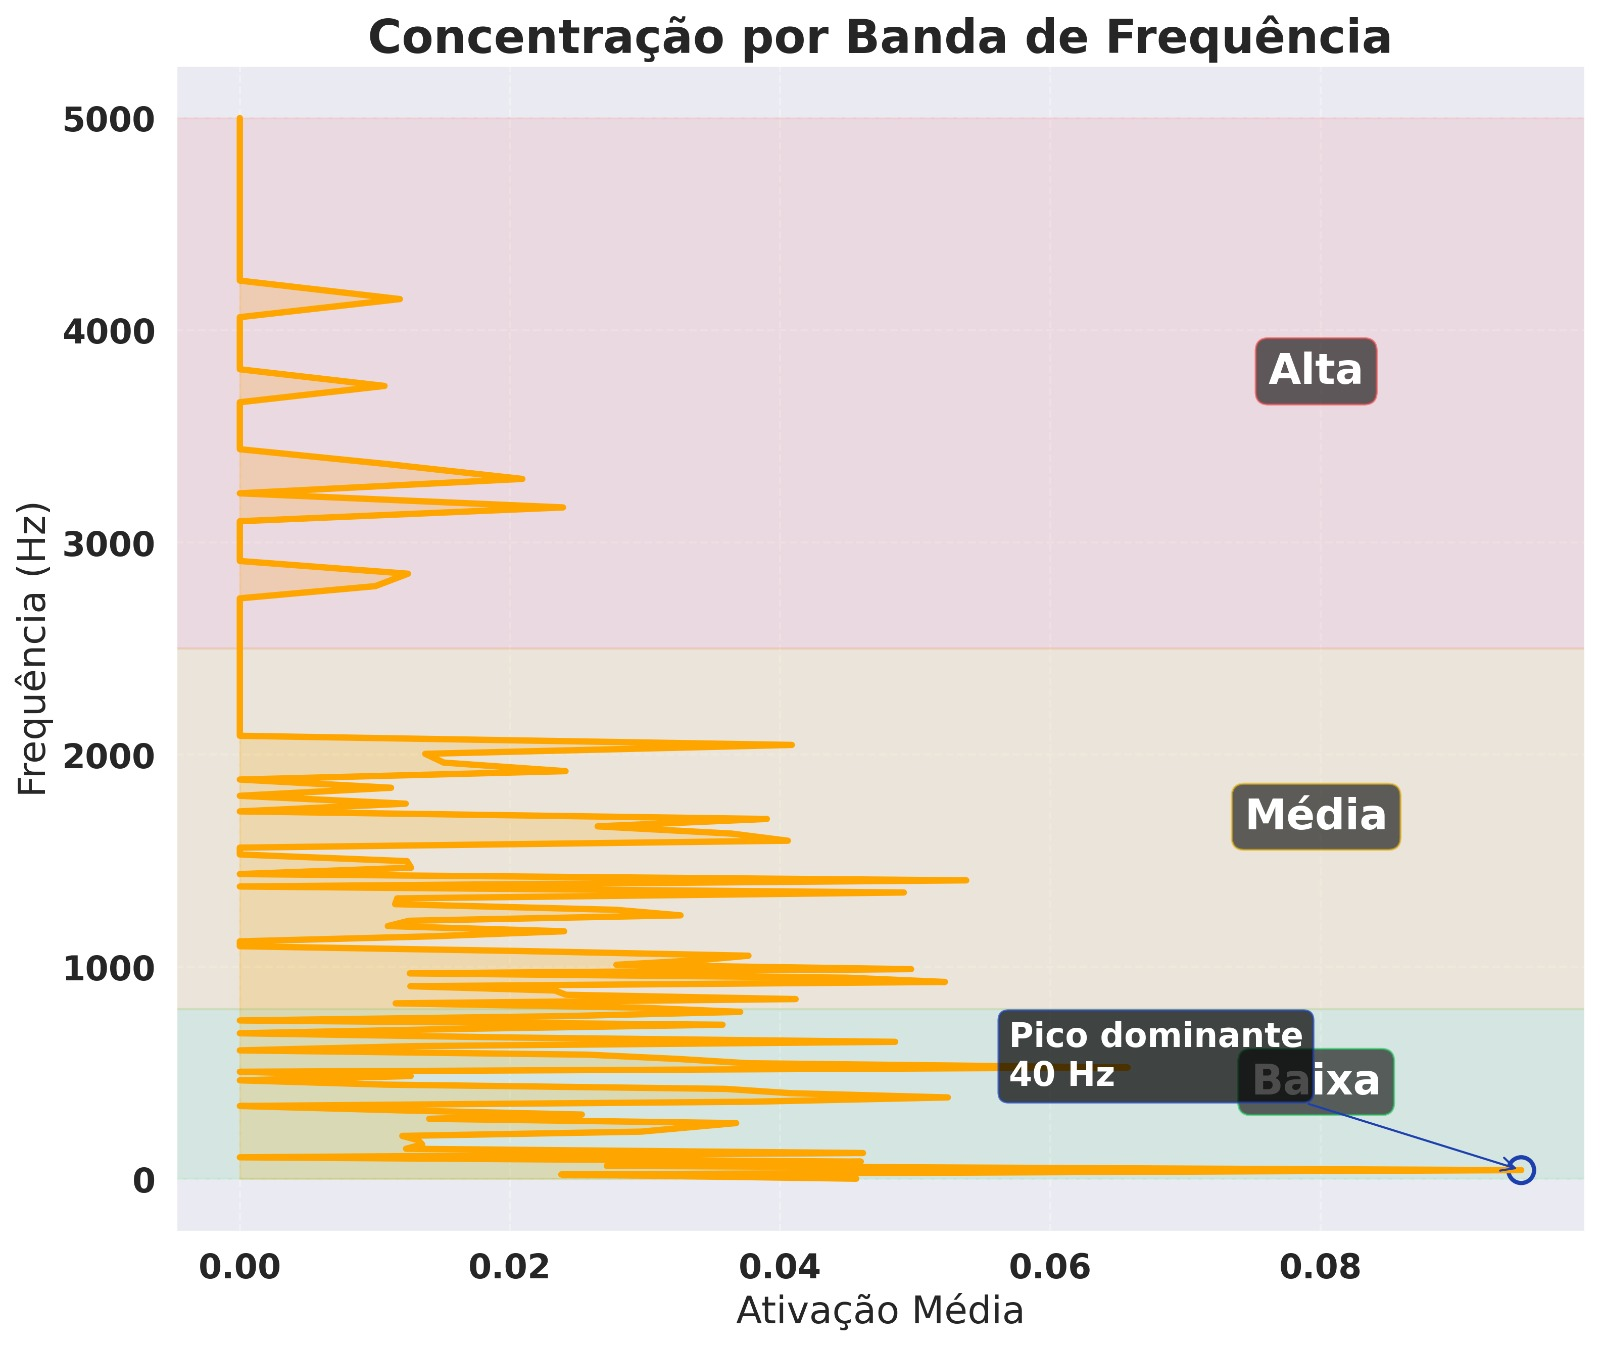
\includegraphics[width=0.94\columnwidth]{images/xai_features.jpg}
    \caption{Distribuição da ativação de anomalia por bandas de frequência, com predominância nas faixas baixa e média.}
    \label{fig:xai_features}
\end{figure}

A convergência entre o mapa temporal (Figura~\ref{fig:xai_heatmap}) e o perfil espectral
(Figura~\ref{fig:xai_features}) comprova que a arquitetura identifica fenômenos físicos reais ---
não artefatos espúrios. A capacidade de sintetizar o diagnóstico em metadados leves (Tabelas~\ref{tab:xai_hotspots}--\ref{tab:xai_bandas}) resolve o gargalo de largura de banda em redes de
chão de fábrica: o dispositivo de borda transmite apenas os metadados, não o áudio bruto~\cite{Uzel2026}.

\subsection{Estratégia de Augmentation (Mixup)}

A Figura~\ref{fig:mixup_strategy} ilustra a estratégia de Mixup adotada para endurecimento da fronteira
de decisão em domain shift.

\begin{figure}[H]
    \centering
    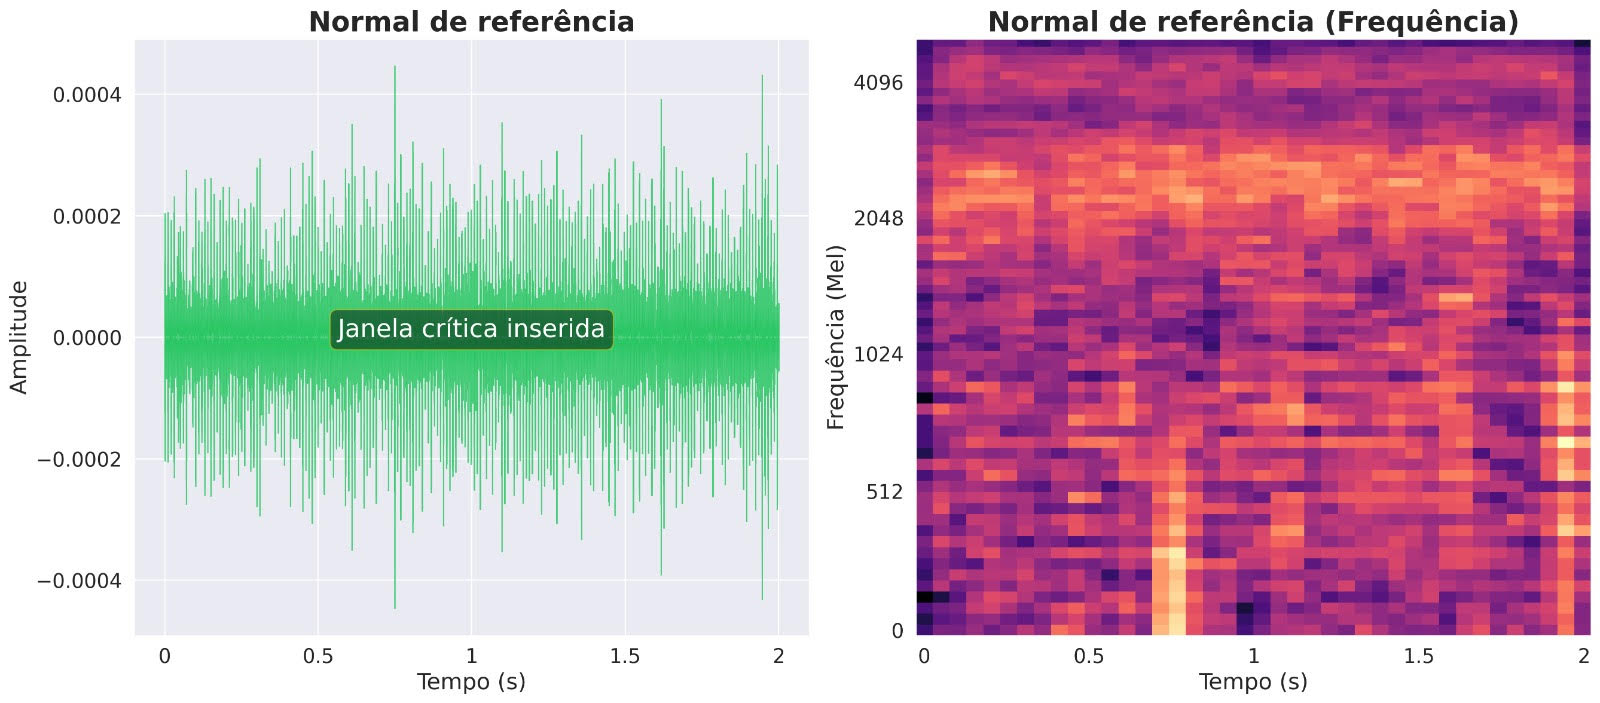
\includegraphics[width=0.9\columnwidth]{images/arquitetura_mixup1.1.jpg}\\[-3pt]
    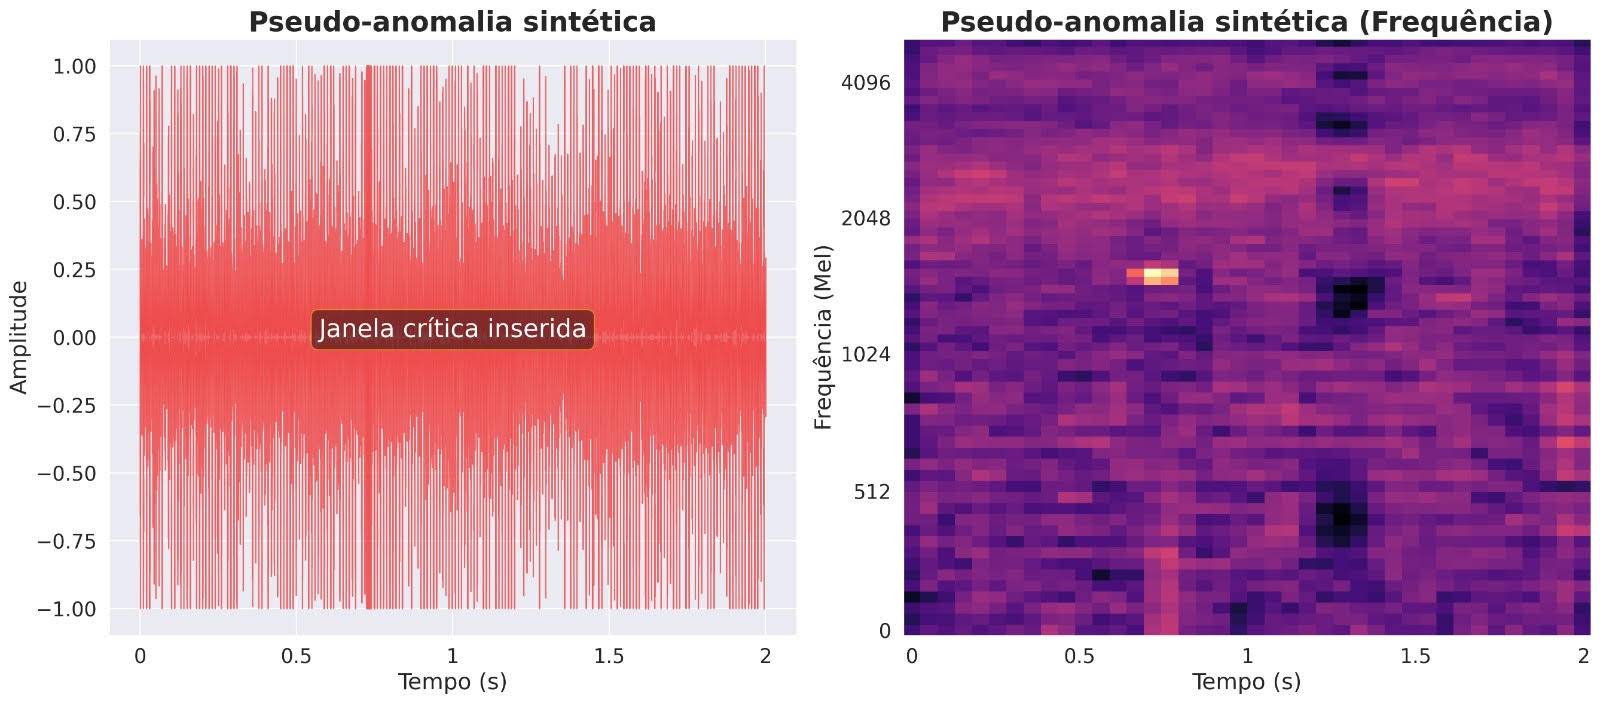
\includegraphics[width=0.9\columnwidth]{images/arquitetura_mixup1.2.jpg}\\[-3pt]
    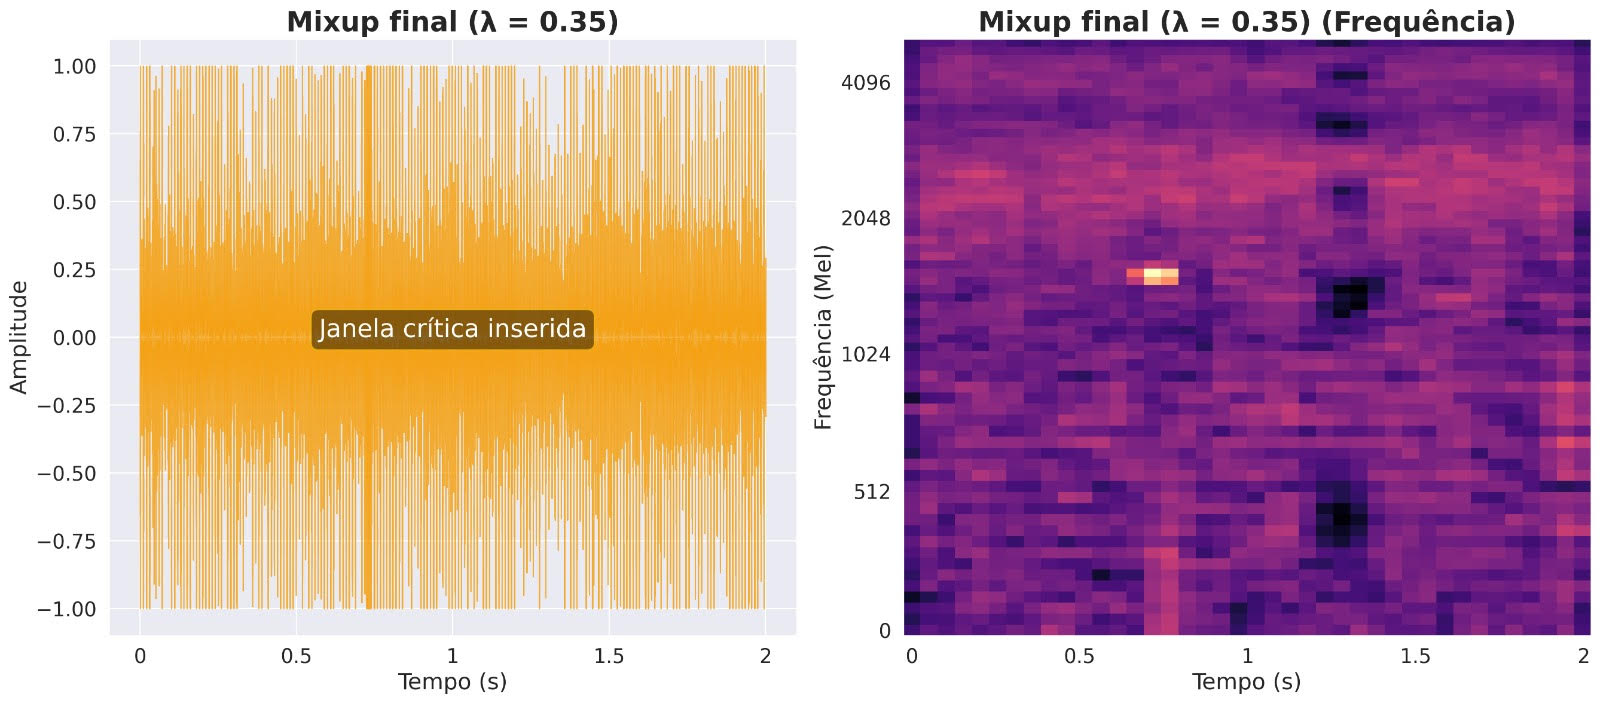
\includegraphics[width=0.9\columnwidth]{images/arquitetura_mixup1.3.jpg}
    \caption{Estratégia Mixup ($\alpha{=}0{,}4$): interpolação convexa entre amostras para generalização de domínio e robustez a variações de sensor.}
    \label{fig:mixup_strategy}
\end{figure}

\color{black}

\section{Discussão}
\color{black}

\subsection{A Regra Fundamental: Pipeline $>$ Modelo}

O resultado central deste trabalho corrobora e estende os achados de~\cite{Khamaisi2025}: em AAD com
dados escassos e restrições de Edge Computing, a \textbf{qualidade do pipeline de processamento supera
a complexidade do modelo}. O XGBoost com Super-Vetor bem construído supera o Tiny-AST --- Transformer
de última geração --- nas métricas DCASE-alinhadas, ao custo de $1/12$ da memória e $1/6$ da latência.
O erro NMF implementa o conceito do Autoencoder em $<0{,}5$~MB e $<5$~ms, eliminando a necessidade da
arquitetura pesada sem penalidade de performance.

\subsection{Por que Deep Learning foi Descartado como Motor}

Todos os modelos de Deep Learning testados foram descartados ou rebaixados a função auxiliar por ao
menos um dos critérios:
\begin{enumerate}
    \item \textbf{Latência:} 45--120~ms, violando o limite de 50~ms para Edge.
    \item \textbf{Memória:} 3--12~MB, violando o limite de 4~MB para TinyML.
    \item \textbf{Overfitting ao domínio:} Com dados escassos, redes profundas memorizam
    características do microfone (sensor-specific features) em vez das da falha mecânica, causando
    colapso em domain shift~\cite{Harada2023}.
\end{enumerate}

\subsection{Por que pAUC@0.1 Muda o Ranking}

A substituição de F1-Score e AUC global por pAUC@FPR~0.1 é uma das contribuições metodológicas mais
relevantes. Em sistemas de alarme industrial, a taxa de falso positivo deve ser minimizada --- um
sistema que gera 10~alarmes falsos por turno perde confiança operacional em semanas. O pAUC@0.1 mede
exclusivamente a performance na região crítica. Este deslocamento de métrica alterou o ranking: Tiny-AST
(excelente em AUC global, pAUC~0,91) caiu para 3º; XGBoost+HHT (ótimo na região de baixo FPR,
pAUC~0,94) ascendeu ao 1º.

\subsection{Protocolo LOSO e Anti-Leakage}

A maioria dos trabalhos de AAD na literatura usa split aleatório ou k-fold padrão, que permitem
vazamento de informação entre sensores/domínios. O protocolo LOSO proposto garante que o modelo nunca
viu dados do sensor de teste, medindo generalização real --- condição necessária para deployment
industrial seguro~\cite{Nishida2025}.

\subsection{Limite Operacional Documentado}

O Protocolo~B falha no cenário MIMII Slider com SNR~$-6$~dB (pAUC~0,79~$<$~0,80). Este é o
\textbf{limite operacional formal}: em ambientes com SNR~$<-3$~dB sem rótulos de anomalia,
o Protocolo~A é obrigatório ou deve-se coletar exemplos de falha.

\color{black}

\color{black}

\section{Conclusão}

Este trabalho apresentou, implementou e validou a arquitetura \textbf{DIAMOND CRISTAL CLEAN} --- uma
pipeline evolutiva dual para Detecção Acústica de Anomalias em ambientes industriais, comprovadamente
viável para Edge Computing e TinyML. A metodologia baseada em 28~experimentos com quatro fases de
desenvolvimento produziu seis achados principais:

\begin{enumerate}
    \item \textbf{HHT+UKF é o componente mais crítico:} Sua remoção custa $-7$~p.p. de pAUC@0.1 e
    causa domain shift catastrófico --- resultado inédito na literatura de AAD por ablation formal.

    \item \textbf{Modelo dual é necessário:} Um único modelo não cobre adequadamente os dois regimes
    operacionais. Protocolo~A (XGBoost, pAUC~0,94) e Protocolo~B (GMM+Gamma, pAUC~0,88) são
    complementares e ambos DCASE-Ready.

    \item \textbf{pAUC@0.1 muda o ranking:} F1-Score e AUC global não são métricas adequadas para
    sistemas de alarme industrial. A adoção do pAUC@FPR~0.1 é recomendação desta pesquisa para a
    comunidade de AAD~\cite{Nishida2025}.

    \item \textbf{Deep Learning é auxiliar, não motor:} CNN, LSTM-AE e Tiny-AST são inviáveis como
    motores de inferência em Edge. O Tiny-AST tem valor exclusivo como gerador de embeddings para XAI
    em análise offline (Cloud).

    \item \textbf{Descarte documentado é contribuição:} O registro formal de 10~técnicas descartadas
    com justificativa quantitativa (pAUC, latência, memória) contribui para a comunidade ao mapear o
    espaço de soluções inviáveis --- informação raramente publicada na literatura~\cite{Khamaisi2025}.

    \item \textbf{XAI com diagnóstico físico:} A camada XAI transforma o score de anomalia em
    evidência física interpretável (hotspots temporais, faixas espectrais, mecanismo provável),
    tornando o sistema auditável para equipes de manutenção~\cite{Ali2025, Zamorano2025}.
\end{enumerate}

O sistema atende plenamente aos três critérios de Edge Computing: pAUC@0.1~$>$~0,80, latência~$<$~50~ms
e memória~$<$~4~MB. O limite operacional documentado --- Protocolo~B falha com SNR~$<-3$~dB sem rótulos
--- fornece diretriz clara para deployment industrial.

Como trabalho futuro, a submissão formal ao DCASE~2025 Task~2 consolidará o posicionamento da
arquitetura no estado da arte internacional, e a integração com firmware de microcontrolador ARM
Cortex-M validará o Cenário~3 em hardware embarcado real~\cite{Uzel2026}.

\color{black}


\bibliographystyle{plain}
\bibliography{refs.bib}

\end{multicols*}

\end{document}
